% !TEX root = main.tex
% Appendix. A: formal setup. B: executors. C: proofs of Theorems 1-3, with numerical checks.
% D: proof of Theorem 4 (joint gradient flow). E: experiments. F: reproducibility.
\providecommand{\reg}[1]{\ensuremath{\mathsf{#1}}}

\section{Formal setup}
\label{app:formal}

This section states the definitions and assumptions that the main text summarizes.

\paragraph{Losses and degree.}

\begin{definition}[Outcome and step losses]
\label{def:losses}
Let $\bm z_t(\bm\theta)\in\R^K$ be the state logits at the position that predicts $s_t$, and $\bm z_{\bm\theta}$
those at the answer position. The \emph{outcome loss} is $\Lout(\bm\theta)=\E[-\log\softmax(\bm z_{\bm\theta})_y]$, and $\bm y=\bm e_y$ is the one-hot answer.
Write $\ell_t(\bm\theta)=\E[-\log\softmax(\bm z_t(\bm\theta))_{s_t}]$. The first state prediction is a boundary case: the previous
count $s_0$ sits in the prompt rather than at the predicting position. The \emph{step loss} is therefore the teacher-forced
transition loss
\[
 \Lstep(\bm\theta)=\frac{1}{n-1}\sum_{t=2}^n\ell_t(\bm\theta),
\]
and $\Lstep^{\mathrm{all}}(\bm\theta)=\tfrac{1}{n}\sum_{t=1}^n\ell_t(\bm\theta)$ also includes $t=1$.
\end{definition}

\begin{definition}[Degree]
\label{def:degree}
Fix the start count. The Hoeffding--Efron--Stein (ANOVA) component $f_S$ of a square-integrable function $f$ of the letters has
\emph{degree} $|S|$, and $(f)_r=\sum_{|S|=r}f_S$. Vector- and matrix-valued functions are decomposed entrywise.
\end{definition}
For centred match bits, a sum has degree $1$ and a product of two distinct bits has degree $2$.
Degree counts input letters, not powers of parameters. Write $A_r:=\E[\|(\bm y-\bm u)_r\|^2]$ and $J_r(\bm\theta):=\E[\|(\Jz)_r\|_F^2]$ as in \cref{eq:credit-degree}; the
\emph{interaction credit} is the credit at degrees $r\ge2$, and $\outcredit=\cred_{\bm y-\bm u}$. With the state-only predictor
$\bm q_s$ and the rule signal $\bm g_t$ of \cref{sec:setting}, $\rulecredit=\E_t\E[\langle\bm z_t,\bm g_t\rangle]$ with $t$ uniform on $\{2,\ldots,n\}$.

\paragraph{Architecture and initialization.}

\begin{assumption}[Architecture]
\label{ass:arch}
A causal Transformer with two blocks of softmax heads and ReLU MLPs, learned token and position
embeddings, a learned relative position bias $\beta_{i-j}$ added to every attention score and initialized at zero, no
LayerNorm, any widths (residual $d_{\mathrm{res}}$, head $d_{\mathrm h}$, MLP $w$) and a linear readout $\mathbf V$;
every logit vector is $\bm z=\mathbf V\bm h$ with $\bm h$ independent of $\mathbf V$. A head may have a fixed, input-independent causal submask;
ordinary attention uses the full prefix.
\end{assumption}

\begin{assumption}[Initialization]
\label{ass:init}
\emph{Scale.} $\bm\theta_0=\initscale\tilde{\bm\theta}$ with $\initscale\le\initscale_0:=c\min(1,\frac{1}{N_b})$, where every weight matrix and embedding block of $\tilde{\bm\theta}$ has operator norm
at most $a_0$ and the value-token embeddings have smallest singular value at least $\embconst>0$.

\emph{Biases.} Every MLP bias satisfies $|\tilde b_m|\ge1$, and each MLP bias vector has norm at most $N_b$.

\emph{Neighbourhood.} We work on
$\initball=\{\bm\theta:\|\bm\theta-\bm\theta_0\|\le\ballradius\initscale,\ \beta=0\}$ with $\ballradius=\min(\frac{1}{8},\frac{\embconst}{4})$, where $\beta$ is the
relative position bias.
\end{assumption}

\begin{assumption}[Task]
\label{ass:task}
The task is counting modulo $K\ge2$ (\cref{def:task}), so $\mixrate<1$.
\end{assumption}

\paragraph{Constants and widths.} On $\initball$, no ReLU unit changes sign (\cref{app:network}). Constants $c,C>0$ depend only on $a_0$, $\embconst$, $K$
and the numbers of blocks and heads, never on the widths, $n$, $\initscale$ or the time. Fan-in-scaled initialization
satisfies \cref{ass:init} w.h.p.\ at every width, with $a_0$ bounded in terms of the largest block aspect ratio,
$\embconst\ge\tfrac{1}{2}$ and $N_b\le2\sqrt w$, provided the MLP biases are drawn with $|\tilde b_m|\in[1,2]$, which default
initializations (zero or small biases) do not do; at the executor width the aspect ratios are bounded, so the theorems
hold there with $n$-independent constants for $\initscale\le c\min(\mixrate,n^{-1/2})$ (\cref{rem:end-width}).

\paragraph{Parameters and training.}

\begin{assumption}[Training]
\label{ass:gd}
Full-batch gradient flow $\tfrac{d\bm\theta}{dt}=-\mathbf P\nabla_{\bm\theta}\mathcal L(\bm\theta)$ on $\Lout$ or $\Lstep$, where $\mathbf P$ is the orthogonal projection onto
the trainable parameter blocks, with the relative
position bias held at its zero initialization. \Cref{thm:outcome-end} drops this restriction and lets the bias train (\cref{lem:bias-uniform}).
\end{assumption}

\label{rem:norms}Parameters carry the Euclidean norm of the vectorized parameters (Frobenius on
each block). In \cref{thm:main,thm:separation} the relative bias is fixed at zero, which is what $\beta=0$ in $\initball$ and
\cref{ass:gd} encode, and $\bm\theta$ denotes the parameters other than $\beta$: the Jacobian $\Jz$, the gradients $\nabla_{\bm\theta}\mathcal L$ and
$\nabla_{\bm\theta}\cred$, and the degree spectra $J_r$ are taken with respect to these parameters only. The step-credit bounds use uniform
zero-score attention through \cref{prop:network}(iv) and do not cover a trained bias. \Cref{thm:outcome-end} allows the bias to be
trained: its proof uses only the logit bounds, which hold for every $\beta$ (\cref{lem:bias-uniform}). The runs of \cref{tab:reach} also train it; the gate head of \cref{thm:joint} has no relative bias. The in-regime runs of \cref{app:exp-regime} have no relative bias.


\section{Exact two-block executors}
\label{app:architectures}

This section proves \cref{prop:represent}. An implementation of the construction is in the accompanying code repository.

\paragraph{Architecture.}
\label{app:construction}
\label{app:model}
Each block has three heads with $d_{\mathrm h}=2n+6$ (the number of positions) and one ReLU MLP of width $\max\{|\Sigma|,3K(n+1),2n+1\}$;
there is no LayerNorm:
\begin{align*}
 \bm h_i&\leftarrow \bm h_i+\sum_{h=1}^{3}\sum_{j\le i}\operatorname{softmax}_{j\le i}\Bigl(\tfrac{1}{\sqrt{d_{\mathrm h}}}(\mathbf W^{(h)}_Q\bm h_i)^{\!\top}\mathbf W^{(h)}_K\bm h_j\Bigr)\mathbf W^{(h)}_V\bm h_j,\\
 \bm h_i&\leftarrow \bm h_i+\mathbf W_{\mathrm{out}}\relu(\mathbf W_{\mathrm{in}}\bm h_i+\bm b_{\mathrm{in}}),\qquad \mathrm{logits}_i=\mathbf V\,\bm h_i .
\end{align*}

\paragraph{Registers.} The residual stream is the concatenation of one-hot registers
\[
 \underbrace{\reg{tl}}_{|\Sigma|}\ \underbrace{\reg{tv}}_{K}\ \underbrace{\reg{pos}}_{d_{\mathrm h}}\ \underbrace{\reg{qry}}_{|\Sigma|}\ \underbrace{\reg{match}}_{1}\
 \underbrace{\reg{prev}}_{K}\ \underbrace{\reg{mt}}_{1}\ \underbrace{\reg{cnt}}_{1}\ \underbrace{\reg{s0}}_{K}\ \underbrace{\reg{out}}_{K},
 \qquad d_{\mathrm{res}}=2|\Sigma|+4K+d_{\mathrm h}+3 .
\]
$\reg r[a]$ is coordinate $a$ of register $\reg r$, and $\mathbf E_{\reg a\leftarrow\reg b}$ copies $\reg b$ into $\reg a$.

\paragraph{Layout.} Token ids: letters $0,\ldots,|\Sigma|-1$, value $v\mapsto|\Sigma|+v$, then SEP, ``:'', EOS. Positions ($0$-indexed):
\[
\begin{array}{ll}
 \text{prompt} & s_0@0,\quad w^\star@1,\quad w_t@(1+t),\quad \mathrm{SEP}@(n+2)\\
 \text{step row} & s_t@(n+2+t),\quad ``{:}"@(2n+3),\quad s_n@(2n+4)\\
 \text{outcome row} & ``{:}"@(n+3),\quad s_n@(n+4)
\end{array}
\]
Position $i$ predicts the token at $i+1$: $n+1+t$ predicts $s_t$, and $n+3$ predicts $s_n$ in the outcome row.

\paragraph{Programs.} State arithmetic is modulo $K$.
\begin{center}\small
\fitwidth{\begin{tabular}{@{}lll@{}}
\toprule
 & step executor & outcome executor\\
\midrule
block 1, head 1 & \multicolumn{2}{l}{$\reg{qry}\leftarrow$ the query, at every letter}\\
block 1, MLP & \multicolumn{2}{l}{$\reg{match}\leftarrow b_t$}\\
block 2, head 1 & $\reg{prev}\leftarrow\widetilde s_{t-1}$ & $\reg{cnt}\leftarrow$ mean of $\reg{match}$ over the letters\\
block 2, head 2 & $\reg{mt}\leftarrow\reg{match}$ of letter $t$ & $\reg{s0}\leftarrow s_0$\\
block 2, head 3 & copy the last displayed count to the answer position & ---\\
block 2, MLP & $\reg{out}\leftarrow\mathrm{lookup}(\reg{prev},\reg{mt})$ & $\reg{out}\leftarrow\mathrm{lookup}(\reg{s0},\reg{cnt})$\\
\bottomrule
\end{tabular}}
\end{center}

\paragraph{Route and average.} Let $\Omega_n=\max\{16,3\log(8(n+3))\}$, $C_Q=\Omega_n\sqrt{d_{\mathrm h}}$, and let $\mathrm{src}(i)\subseteq\{0,\ldots,i\}$ be the source set
of position $i$ (a fallback $\{f\}$ where none is listed). Set
\begin{equation}
 \begin{gathered}
 (\mathbf W_K)_{j,\reg{pos}[j]}=1,\qquad (\mathbf W_Q)_{j,\reg{pos}[i]}=C_Q\ \ (j\in\mathrm{src}(i)),\\
 \tfrac{1}{\sqrt{d_{\mathrm h}}}(\mathbf W_Q\bm h_i)^\top \mathbf W_K\bm h_j=\Omega_n\,[j\in\mathrm{src}(i)] .
 \end{gathered}
 \label{eq:route}
\end{equation}
With $\mathbf W_V=\mathbf E_{\reg a\leftarrow\reg b}$, the head writes into $\reg a$ the average of $\reg b$ over $\mathrm{src}(i)$, up to the leak bounded below; $|\mathrm{src}(i)|=1$ is a
route and $|\mathrm{src}(i)|>1$ an average. A fallback $f>i$ gives uniform attention at a position with no supervised prediction.

\paragraph{Lookup.} For a count $s$ and a bit $b\in\{0,1\}$, use one unit per pair $(s',b')$ with
\[
 \mathrm{pre}_{s'b'}=[s=s']+[b=b']-\tfrac{3}{2}=\begin{cases}\tfrac{1}{2}&(s',b')=(s,b),\\\le-\tfrac{1}{2}&\text{otherwise},\end{cases}
\]
and output weights $2\bm e_{s'+b'}$:
\begin{equation}
 \textstyle\sum_{s',b'}2\,\bm e_{s'+b'}\relu(\mathrm{pre}_{s'b'})=\bm e_{s+b}.
 \label{eq:lookup}
\end{equation}

\subsection{Both programs are exact}
\label{app:exact}

\begin{proof}[Proof of \cref{prop:represent}]
\emph{Ideal routing} ($\Omega_n=\infty$). With $m=\sum_tb_t$ and $[m=a]=\relu(m-a+1)-2\relu(m-a)+\relu(m-a-1)$,
\begin{gather*}
 \reg{match}_{1+t}=2\textstyle\sum_{a\in\Sigma}\relu\bigl([w_t=a]+[w^\star=a]-\frac{3}{2}\bigr)=b_t,\\
 \reg{prev}_{n+1+t}=\bm e_{s_{t-1}},\qquad \reg{mt}_{n+1+t}=b_t,\qquad
 \reg{cnt}_{n+3}=n\cdot\tfrac{1}{n}\textstyle\sum_tb_t=m,\qquad \reg{s0}_{n+3}=\bm e_{s_0},\\
 \reg{out}_{n+1+t}=\sum_{j,\iota}\bm e_{j+\iota}\,2\relu\Bigl([s_{t-1}=j]+[b_t=\iota]-\frac{3}{2}\Bigr)=\bm e_{s_t},\\
 \reg{out}_{n+3}=\sum_{j,a}\bm e_{j+a}[s_0=j][m=a]=\bm e_{s_n}.
\end{gather*}
The test $[s_0=j]$ is applied by adding $(n+2)([s_0=j]-1)$ to each of the three pre-activations of $[m=a]$. The readout has weight $20$
on $\reg{out}$ for value tokens and weight $20$ on the relevant $\reg{pos}$ coordinates for ``:'' and EOS; all unused maps are zero.

\emph{Finite scores.} A row puts total weight at most $\omega^{\mathrm{leak}}_n$ outside its sources, where
\[
 \omega^{\mathrm{leak}}_n=(d_{\mathrm h}-1)e^{-\Omega_n}<\frac{2(n+3)}{(8(n+3))^3}=\frac{1}{256(n+3)^2}.
\]
Hence
\begin{gather*}
 |\reg{match}-b_t|\le2\omega^{\mathrm{leak}}_n,\qquad \|\reg{prev}-\bm e_{s_{t-1}}\|\le\omega^{\mathrm{leak}}_n,\qquad |\reg{mt}-b_t|\le3\omega^{\mathrm{leak}}_n,\\
 |\reg{cnt}-m|\le3n\,\omega^{\mathrm{leak}}_n,\qquad \|\reg{s0}-\bm e_{s_0}\|\le\omega^{\mathrm{leak}}_n .
\end{gather*}
At the step positions,
\[
 \mathrm{pre}_{s_t}\ge\tfrac{1}{2}-4\omega^{\mathrm{leak}}_n>0>\max_{a\ne s_t}\mathrm{pre}_a,\qquad \reg{out}_{s_t}\ge1-8\omega^{\mathrm{leak}}_n .
\]
At the answer position the errors add to $(4n+2)\omega^{\mathrm{leak}}_n<\frac{1}{192}$, and the three-ReLU test is $1$-Lipschitz, so
\[
 \reg{out}_{s_n}\ge1-(4n+2)\omega^{\mathrm{leak}}_n,\qquad \max_{a\ne s_n}\reg{out}_a\le(4n+2)\omega^{\mathrm{leak}}_n .
\]
With readout weight $20$ and $a^\star$ the gold token at a supervised position,
\[
 z_{a^\star}-\max_{a\ne a^\star}z_a\ge20\min\bigl\{1-8\omega^{\mathrm{leak}}_n,\ 1-2(4n+2)\omega^{\mathrm{leak}}_n\bigr\}>19 .
\]

\emph{Open neighbourhood.} Let $\mathcal P_n$ be the finite set of gold prefixes and supervised positions. By continuity there is
$r_{\mathrm{exec},n}>0$ with
\[
 \|\bm\theta-\bm\theta^\star\|<r_{\mathrm{exec},n}\implies\max_{P\in\mathcal P_n}\|\bm z_{\bm\theta}(P)-\bm z_{\bm\theta^\star}(P)\|_\infty<\tfrac{19}{2},
\]
so every greedy prediction is $a^\star$, and induction over the continuation gives the claim.
\end{proof}


\section{Proofs of \texorpdfstring{\cref{thm:main,thm:separation,thm:outcome-end}}{Theorems 1-3}}
\label{app:damping-proof}
\label{app:mainproofs}

\subsection{Conventions and degree calculus}
\label{app:assumptions}

\begin{table}[h]
\caption{Lemmas of \cref{app:mainproofs} and the theorems they feed.}
\label{tab:C-map}
\centering\small
\fitwidth{\begin{tabular}{@{}lll@{}}
\toprule
Result & Key estimate & Feeds\\
\midrule
\ref{lem:gradient-split} & $\nabla_{\bm\theta}\Lout$ splits; answer-dependent part $\le\sqrt{(A_0+A_1)(J_0+J_1)}+\sqrt{\textstyle\sum_{r\ge2}J_r}$ & \cref{thm:main}\\
\ref{lem:target-contraction} & $\E\|(\bm y-\bm u)_S\|^2\le\mixrate^{2(n-|S|)}$ & \cref{thm:main,thm:outcome-end}\\
\ref{prop:score-degree} & $\mathbf J^{[0]}_S=0$ for $|S|\ge2$; $\ \sum_S\sup\|\mathbf J^{[k]}_S\|_F\le C\initscale^2(\attconst\initscale^4)^k$, $|S|\le2k+1$ & \cref{thm:main,thm:outcome-end}\\
\ref{lem:score-sum} & interaction credit $\le C\initscale^6\mixrate^{n-3}$; $\ |\outcredit|\le C\initscale^2\mixrate^n$ & \cref{thm:main,thm:outcome-end}\\
\ref{lem:bias-uniform}, \ref{lem:end-smooth} & bounds uniform in $\beta$; $\|\nabla_{\bm\theta}\Lout\|\le C_1\initscale$, curvature $\le C_1$ & \cref{thm:outcome-end}\\
\ref{lem:dilution-average}--\ref{lem:leading} & rule credit needs letter and state; $\E_t[\kappa_{l_t,i_t}]\le\frac{6}{n}$; leading coefficient $\initscale^6P_n$ & \cref{thm:separation}\\
\bottomrule
\end{tabular}}
\end{table}


(A1)--(A4) denote \cref{ass:arch,ass:init,ass:task,ass:gd}, and (A3$'$) a uniform start. Unless stated otherwise the query and the start
count are fixed. Constants $c,C$ depend only on $a_0,\embconst,K$ and the numbers of blocks and heads. Every bound stated on $\initball$ also
holds on $\initball'=\{\bm\theta:\|\bm\theta-\bm\theta_0\|\le2\ballradius\initscale,\ \beta=0\}$, whose relative radius is at most $\min(\frac{1}{4},\frac{\embconst}{2})$; there
$|b_m|\ge\frac{\initscale}{2}$ and $\sigma_{\min}(\mathbf E_{\mathrm{val}})\ge\frac{\initscale\embconst}{2}$. The only width-dependent threshold is $\initscale_0=c\min(1,\frac{1}{N_b})$.

\paragraph{The bias condition.}\label{rem:two-block-bias} The bias condition of (A2) fixes one ReLU pattern for all inputs on $\initball$. The AdamW runs violate it: at their initialization
($n=8$, MLP width $54$, $\initscale=0.02$, Gaussian biases), $10$ to $19$ of the $54$ units per block switch with the letters. Those
runs therefore lie outside the regime of the theorems; \cref{app:exp-regime} repeats the key measurements inside it.


\paragraph{Degree calculus.} For $L^2$ functions of independent letters \citep{hoeffding1948class,efron1981jackknife,odonnell2014analysis},
$f=\sum_Sf_S$ with $f_S=\sum_{U\subseteq S}(-1)^{|S\setminus U|}\E[f\mid w_U]$; the components are orthogonal, $f_S$ is centred in each letter of
$S$, and $f_S=0$ unless $S\subseteq U$ when $f$ depends only on $w_U$. For matrix-valued $f$ and vector-valued $g$, orthogonality and
Cauchy--Schwarz give
\begin{gather}
 \E[f^\top g]=\sum_S\E[f_S^\top g_S]=\sum_{r=0}^n\E[f_r^\top g_r],
 \nonumber\\
 \bigl\|\E[f_r^\top g_r]\bigr\|\le\Bigl(\sum_{|S|=r}\E\|f_S\|_F^2\Bigr)^{1/2}\Bigl(\sum_{|S|=r}\E\|g_S\|^2\Bigr)^{1/2}.
 \label{eq:matching}
\end{gather}
At $\bm p=\bm u$, $-\nabla_{\bm\theta}\Lout=\E[(\Jz)^\top(\bm y-\bm u)]$, and \cref{eq:matching} with $f=\Jz$, $g=\bm y-\bm u$ is \cref{eq:credit-degree}.

\begin{lemma}[Gradient split]
\label{lem:gradient-split}
For every differentiable model under the independent-letter law, with $\outcredit(\bm\theta)=\E[\langle\bm z_{\bm\theta},\bm y-\bm u\rangle]$,
\begin{gather*}
 \nabla_{\bm\theta}\Lout=\underbrace{\E\bigl[(\Jz)^\top(\bm p-\bm u)\bigr]}_{\text{answer-independent}}-\underbrace{\nabla_{\bm\theta}\outcredit}_{\text{answer-dependent}},\\
 \Bigl\|\nabla_{\bm\theta}\outcredit\Bigr\|\le\sqrt{(A_0+A_1)(J_0+J_1)}+\sqrt{\bigl(1-\tfrac{1}{K}\bigr)\textstyle\sum_{r\ge2}J_r}.
\end{gather*}
\end{lemma}

\begin{proof}
$\bm p-\bm e_y=(\bm p-\bm u)-(\bm y-\bm u)$ gives the split, and $\nabla_{\bm\theta}\outcredit=\E[(\Jz)^\top(\bm y-\bm u)]$. By \cref{eq:matching} and Cauchy--Schwarz over
$r\in\{0,1\}$ and over $r\ge2$,
\[
 \|\nabla_{\bm\theta}\outcredit\|\le\sum_{r\le1}\sqrt{A_rJ_r}+\Bigl(\sum_{r\ge2}A_r\Bigr)^{1/2}\Bigl(\sum_{r\ge2}J_r\Bigr)^{1/2},\qquad \sum_rA_r=\E\|\bm y-\bm u\|^2=1-\tfrac{1}{K} .
\qedhere
\]
\end{proof}

\subsection{Target spectrum}
\label{app:target-spectrum}

\paragraph{Contraction and spectra.}\label{app:contraction} By \cref{eq:lambda}, $\mixrate^2=1-2p(1-p)(1-\cos\tfrac{2\pi}{K})$, and for $K=2$,
$\mixrate=|1-2p|$ and $1-\mixrate^2=4p(1-p)$. With $\alpha=e^{2\pi\mathrm i/K}$ and the Fourier multipliers
$\rho_j=1-p+p\alpha^j$, so that $\mixrate=\max_{j\ne0}|\rho_j|$, one unseen letter multiplies each nonconstant count
mode $\alpha^{js_t}$ by $\rho_j$, while one displayed transition keeps the innovation
\begin{equation}
 \E\bigl[\bigl|\alpha^{j s_t}-\rho_j\,\alpha^{j s_{t-1}}\bigr|^2\bigr]=1-|\rho_j|^2\ge1-\mixrate^2 .
 \label{eq:move-variance}
\end{equation}
In the Fourier basis of $\one^\perp$, $\operatorname{Cov}(\bm g_t)$ is diagonal with entries $\tfrac{1}{K}(1-|\rho_j|^2)=\tfrac{2p(1-p)}{K}\bigl(1-\cos\tfrac{2\pi j}{K}\bigr)$,
which gives \cref{eq:local-variation}. Hence every set $S$ of letters has
\begin{equation}
 \E\bigl[\|(\bm y-\bm u)_S\|^2\bigr]\le\left(1-\frac{1}{K}\right)\mixrate^{2(n-|S|)}
 \label{eq:horizon}
\end{equation}
(\cref{lem:target-contraction}).

\begin{lemma}[Exact target spectrum]
\label{lem:target-contraction}
Assume (A3) and fix the start count. For every $S\subseteq[n]$ and $0\le r\le n$,
\begin{align*}
 \E\|(\bm y-\bm u)_S\|^2&=\frac{1}{K}\sum_{j=1}^{K-1}|\rho_j|^{2(n-|S|)}(1-|\rho_j|^2)^{|S|}\le\Bigl(1-\frac{1}{K}\Bigr)\mixrate^{2(n-|S|)},\\
 A_r&=\binom nr\frac{1}{K}\sum_{j=1}^{K-1}|\rho_j|^{2(n-r)}(1-|\rho_j|^2)^r\le\binom nr\Bigl(1-\frac{1}{K}\Bigr)\mixrate^{2(n-r)},
\end{align*}
with $0^0=1$.
\end{lemma}

\begin{proof}
$\alpha^{js_n}=\alpha^{js_0}\prod_{t=1}^n\alpha^{jb_t}$ and $\alpha^{jb_t}=\rho_j+(\alpha^{jb_t}-\rho_j)$ with $\E[\alpha^{jb_t}-\rho_j]=0$. Expanding the product,
\begin{equation}
 (\alpha^{js_n})_S=\alpha^{js_0}\rho_j^{\,n-|S|}\prod_{t\in S}(\alpha^{jb_t}-\rho_j),
 \label{eq:product-rep}
\end{equation}
which is centred in each letter of $S$ and hence the Efron--Stein component. By independence and $\E|\alpha^{jb_t}-\rho_j|^2=1-|\rho_j|^2$,
$\E|(\alpha^{js_n})_S|^2=|\rho_j|^{2(n-|S|)}(1-|\rho_j|^2)^{|S|}$. Parseval over the nonconstant modes $j=1,\ldots,K-1$ gives the identity for $S$;
$|\rho_j|\le\mixrate$ and $1-|\rho_j|^2\le1$ give the bound; summing over the $\binom nr$ sets of size $r$ gives $A_r$.
\end{proof}

\paragraph{Sharpness.}\label{rem:tight} The $j=1$ term gives $A_r\ge\frac{\binom nr\mixrate^{2(n-r)}(1-\mixrate^2)^r}{K}$, so the exponent $n-r$ is sharp for $0<\mixrate<1$. The overlap bound
$\sqrt{A_rJ_r}$ is attained by $\bm z_{\bm\theta}=\bm\theta(\bm y-\bm u)_r$. For $K=2$ the normalized spectrum is $\mathrm{Binomial}(n,1-\mixrate^2)$
\citep{odonnell2014analysis}.
\subsection{Model spectrum}
\label{app:model-spectrum}

\paragraph{Score expansion.} For $u\in[0,1]$, let $\bm z(u)$ be the network with every score $\psi_{il}$, in both blocks, replaced by
$u\psi_{il}$. Then $\bm z(1)=\bm z_{\bm\theta}$, and for every integer $k_0\ge0$,
\begin{equation}
 \bm z_{\bm\theta}=\sum_{k=0}^{k_0}\bm z^{[k]}+\bm z_{\mathrm{rem}},\qquad
 \bm z^{[k]}=\frac{1}{k!}\frac{d^k\bm z}{du^k}(0),\qquad
 \bm z_{\mathrm{rem}}=\int_0^1\frac{(1-u)^{k_0}}{k_0!}\frac{d^{k_0+1}\bm z}{du^{k_0+1}}(u)\,du .
 \label{eq:score-split}
\end{equation}
$\mathbf J^{[k]}$ and $\mathbf J_{\mathrm{rem}}$ are the corresponding Jacobian terms, and $\mathbf J^{[k]}_S$ is the Efron--Stein component of $\mathbf J^{[k]}$ on $S$.

\begin{proposition}[Score count and degree]
\label{prop:score-degree}
Fix the start state and the query. For $\bm\theta\in\initball$, $\Jz=\sum_{k=0}^{k_0}\mathbf J^{[k]}+\mathbf J_{\mathrm{rem}}$, and there is $\attconst$ such that:
\begin{enumerate}[label=(\roman*),leftmargin=*,itemsep=2pt,topsep=2pt]
\item $\sup\|\mathbf J^{[0]}\|_F\le C\initscale$, $\ \sum_{|S|=1}\sup\|\mathbf J^{[0]}_S\|_F\le C\initscale^2$, and $\mathbf J^{[0]}_S=0$ for $|S|\ge2$;
\item for $k\ge1$, $\ \sum_S\sup\|\mathbf J^{[k]}_S\|_F\le C\initscale^2(\attconst\initscale^4)^k$, and $\mathbf J^{[k]}_S=0$ for $|S|>2k+1$;
\item $\sup\|\mathbf J_{\mathrm{rem}}\|_F\le C\initscale^2(\attconst\initscale^4)^{k_0+1}$.
\end{enumerate}
The same bounds hold for $\bm z^{[k]}$ and $\bm z_{\mathrm{rem}}$ with one more factor $\initscale$. Suprema are over inputs; constants do not depend on
$n$, $k$ or $k_0$.
\end{proposition}

$\attconst$ is fixed once, large enough for \cref{prop:score-degree,prop:network}; it depends only on $a_0$, $\embconst$ and $K$.

\label{app:network}

\begin{proposition}[Bounds for the score expansion]
\label{prop:network}
Assume (A1)--(A2). Uniformly on $\initball$, at every position and input, with $\bm x_i$ the token-plus-position vector,
$\partial_vF=\frac{d}{ds}F(\bm\theta+sv)|_{s=0}$, and $\|F\|_{\mathrm{abs}}$ the sum of the monomial norm bounds before cancellation:
\begin{enumerate}[label=(\roman*),leftmargin=*,itemsep=1pt,topsep=2pt]
\item with input-independent offsets $\bm O^1=\bm o_1$, $\bm O^2=\bm o_1+\bm o_2$: $\bm h_i^\ell=\bm x_i+\bm O^\ell+O(\initscale^2)$, $|\psi_{il}|\le C\initscale^4$,
$\|\bm z_i\|\le C\initscale^2$, $\|\partial_v\bm z_i\|\le C\initscale\|v\|$;
\item for $k\ge1$, $u\in[0,1]$ and $\|v\|=1$,
\[
 \frac{1}{k!}\Bigl\|\frac{d^k\bm z_i}{du^k}\Bigr\|\le C\initscale^3(C_0\initscale^4)^k,\qquad
 \frac{1}{k!}\Bigl\|\partial_v\frac{d^k\bm z_i}{du^k}\Bigr\|\le C\initscale^2(C_0\initscale^4)^k;
\]
the same holds for the absolute sums at $u=0$, for $\bm h^2_i$ with one power of $\initscale$ fewer, and for the Taylor remainder with $k=k_0+1$;
\item the zero-score network is affine in the inputs; its transported logit terms have tangent $O(\initscale^2)$, and direct-input and
input-free terms have tangent $O(\initscale)$; an order-$k$ coefficient contains at most $2k+1$ inputs; a one-score logit term has size
$O(\initscale^7)$ and tangent $O(\initscale^6)$;
\item with full-prefix attention, the terms of the order-$k$ coefficients at $u=0$ that contain an earlier input $\bm x_l$, $l<i$, obey the
bounds of (ii) multiplied by
\begin{equation}
 \kappa_{l,i}=\frac{1}{m_i}\Bigl(1+\sum_{l<j\le i}\frac{1}{m_j}\Bigr),\qquad m_i=i+1,
 \label{eq:dilution}
\end{equation}
after enlarging $C_0$.
\end{enumerate}
The constants do not depend on $n$, the widths or $k$.
\end{proposition}

\begin{proof}
For a network quantity $F$ let $F^{[k]}(u)=\frac{1}{k!}\frac{d^kF}{du^k}(u)$, so that $\bm z^{[k]}=\bm z^{[k]}(0)$, and write $\|F^{[k]}\|$ for its supremum over
inputs, positions and $u\in[0,1]$ (the $\ell_1$ norm for attention rows).

\emph{(i).} $|b_m|\ge\frac{\initscale}{2}>C\initscale^2\ge|(\mathbf W_{\mathrm{in}}\bm h)_m|$, so one activation matrix $\mathbf D_{\mathrm{act}}$ serves every input and every $u$, and
\[
 \bm h_i^\ell=\mathbf M_\ell\bigl(\bm h_i^{\ell-1}+\bm a_i^\ell\bigr)+\bm o_\ell,\qquad \mathbf M_\ell=\mathbf I+\mathbf W^\ell_{\mathrm{out}}\mathbf D_{\mathrm{act}}\mathbf W^\ell_{\mathrm{in}},\qquad \bm o_\ell=\mathbf W^\ell_{\mathrm{out}}\mathbf D_{\mathrm{act}}\bm b^\ell,
\]
with $\bm a_i^\ell=\sum_{\mathrm{heads}}\sum_{j\le i}\omega_{ij}\mathbf W_V\bm h^{\ell-1}_j$ and $\omega_{i\cdot}=\softmax(u\psi_{i\cdot})$. Then
\[
 \|\mathbf M_\ell-\mathbf I\|\le C\initscale^2,\qquad \|\bm o_\ell\|\le2a_0N_b\initscale^2\le a_0\initscale,\qquad \|\partial_v\bm o_\ell\|\le(a_0+2N_b)\initscale\le C,
\]
and $\|\omega_{i\cdot}\|_1=1$. Induction over the two blocks gives (i).

\emph{Softmax calculus.} For $\omega=\softmax(s)$, $\E_\omega[f]=\sum_j\omega_jf_j$ and a direction $\bm\nu$,
\[
 \tfrac{d}{dt}\omega_j(s+t\bm\nu)\big|_0=\omega_j(\nu_j-\E_\omega[\bm\nu]),\qquad
 \tfrac{d}{dt}\E_{\omega(s+t\bm\nu)}[f]\big|_0=\E_\omega[\bm\nu f]-\E_\omega[\bm\nu]\E_\omega[f].
\]
After $k$ derivatives each term has at most $k+1$ averages and each direction once; the absolute coefficient sums obey $a_{k+1}\le2(k+1)a_k$,
$a_0=1$. By duality,
\begin{equation}
 \bigl\|D^k\omega(s)[\bm\nu_1,\ldots,\bm\nu_k]\bigr\|_1\le2^kk!\prod_a\|\bm\nu_a\|_\infty .
 \label{eq:softmax-avg}
\end{equation}
Normalized derivatives of products are convolutions; those of compositions sum over the $\binom{k-1}{j-1}$ compositions of $k$ into $j$
positive parts. Hence
\[
 \tfrac{1}{j!}\|F^{(j)}\|\le Ac^j,\ \ \|h^{[k]}\|\le ab^k\quad\implies\quad\|(F\circ h)^{[k]}\|\le Aca\,b^k(1+ca)^{k-1}.
\]

\emph{(ii), values.} With $\|\bm\omega^{\ell,[0]}\|_1=1$, $\|\bm h^{0,[k]}\|=0$ for $k\ge1$, and $a_r\ge1$ in the compositions,
\begin{alignat*}{2}
 \|\psi^{\ell,[k]}\|&\le C\initscale^2\textstyle\sum_{a+b=k}\|\bm h^{\ell-1,[a]}\|\,\|\bm h^{\ell-1,[b]}\| &\qquad& \why{score is a product}\\
 \|(u\psi^\ell)^{[k]}\|&\le\|\psi^{\ell,[k]}\|+\|\psi^{\ell,[k-1]}\| && \why{$(u\psi)^{[k]}=u\psi^{[k]}+\psi^{[k-1]}$}\\
 \|\bm\omega^{\ell,[k]}\|_1&\le\textstyle\sum_{j=1}^k2^j\sum_{a_1+\cdots+a_j=k}\prod_r\|(u\psi^\ell)^{[a_r]}\| && \why{composition, \cref{eq:softmax-avg}}\\
 \|\bm a^{\ell,[k]}\|&\le C\initscale\textstyle\sum_{a+c=k}\|\bm\omega^{\ell,[a]}\|_1\,\|\bm h^{\ell-1,[c]}\| && \why{head output is a product}\\
 \|\bm h^{\ell,[k]}\|&\le C\bigl(\|\bm h^{\ell-1,[k]}\|+\|\bm a^{\ell,[k]}\|\bigr) && \why{affine block}\\
 \|\bm z^{[k]}\|&\le C\initscale\,\|\bm h^{2,[k]}\| && \why{readout}
\end{alignat*}
With $b=C\initscale^4$, block $1$ gives $\|\bm\omega^{1,[k]}\|_1\le b^k$ and $\|\bm a^{1,[k]}\|+\|\bm h^{1,[k]}\|\le C\initscale^2b^k$. Then $\|\psi^{2,[0]}\|\le C\initscale^4$,
$\|\psi^{2,[k]}\|\le C\initscale^5(k+1)b^k$ for $k\ge1$, and $\|(u\psi^2)^{[k]}\|\le C(2b)^k$, so
\begin{gather*}
 \|\bm\omega^{2,[k]}\|_1\le C\sum_{j=1}^k\binom{k-1}{j-1}C^j(2b)^k\le C(Cb)^k,\\
 \|\bm a^{2,[k]}\|+\|\bm h^{2,[k]}\|\le C\initscale^2(Cb)^k,\qquad \|\bm z^{[k]}\|\le C\initscale^3(C_0\initscale^4)^k .
\end{gather*}

\emph{(ii), tangents, remainders, absolute sums.} Differentiating along $v$ replaces one factor of each product by its tangent, or one
$(u\psi)^{[a]}$ in a softmax term, or adds $D^{j+1}\omega[\partial_v(u\psi)^{[0]},\ldots]$. With $\|\partial_v\bm h^{0,[0]}\|=O(1)$, $\|\partial_v\psi^{\ell,[0]}\|=O(\initscale^3)$
and $j+1\le2^k$ absorbed into $C_0^k$,
\begin{gather*}
 \|\partial_v\bm\omega^{\ell,[k]}\|_1\le C\initscale^{-1}(C_0\initscale^4)^k,\qquad \|\partial_v\bm a^{\ell,[k]}\|+\|\partial_v\bm h^{\ell,[k]}\|\le C\initscale(C_0\initscale^4)^k,\\
 \|\partial_v\bm z^{[k]}\|\le C\initscale^2(C_0\initscale^4)^k .
\end{gather*}
The integral remainder is bounded by the supremum of the next normalized derivative. At $u=0$,
$\|m^{-1}\sum_j\prod_rF_r(j)\|_{\mathrm{abs}}\le\prod_r\max_j\|F_r(j)\|_{\mathrm{abs}}$, and an order-$k$ monomial has $O(k+1)$ parameter and input
occurrences, so differentiating its norm bound costs at most $\frac{C(k+1)}{\initscale}\le \frac{C2^k}{\initscale}$.

\emph{(iii).} At zero scores the network is affine in the inputs:
\begin{gather*}
 \bm h^1_j=\mathbf M_1\Bigl(\bm x_j+\frac{1}{m_j}\sum_{l\le j}\mathbf W^1_V\bm x_l\Bigr)+\bm o_1,\\
 \bm z^{[0]}_i=\mathbf V\Bigl[\mathbf M_2\Bigl(\bm h^1_i+\frac{1}{m_i}\sum_{j\le i}\mathbf W^2_V\bm h^1_j\Bigr)+\bm o_2\Bigr].
\end{gather*}
Transported terms contain $\mathbf V$, $\mathbf W_V$ and some $\bm x_j$, so their tangent is $O(\initscale^2)$; direct-input and input-free terms have tangent $O(\initscale)$.
With $d(F)$ the number of input occurrences in $F$,
\begin{alignat*}{2}
 d(\bm h^{\ell,[a]})&\le2a+1 &\qquad& \why{induction on $\ell$}\\
 d(\psi^{\ell,[b]})&\le2b+2 && \why{score is a product of two residuals}\\
 d\bigl((u\psi)^{[a]}\bigr)&\le2a && \why{$(u\psi)^{[a]}=\psi^{[a-1]}$}\\
 d(\text{order-$k$ head term})&\le2a_1+\cdots+2a_j+2c+1=2k+1 && \why{$a_1+\cdots+a_j+c=k$}
\end{alignat*}
and affine MLPs and parameter derivatives add none. The one-score correction is
\[
 \frac{1}{m_i}\sum_{j\le i}\bigl(\psi_{ij}(0)-\bar\psi_i(0)\bigr)\mathbf W_V\bm h_j(0),\qquad \bar\psi_i(0)=\frac{1}{m_i}\sum_{l\le i}\psi_{il}(0);
\]
its logit terms contain $\mathbf V,\mathbf W_V,\mathbf W_Q,\mathbf W_K$ and three residual inputs, so they have size $O(\initscale^7)$ and tangent $O(\initscale^6)$.

\emph{(iv).} Fix $l<i$; (iv) concerns the coefficients at $u=0$ and their tangents. Replace $\bm x_l$ by $\chi\bm x_l$. A monomial containing $\bm x_l$
exactly $d\ge1$ times carries $\chi^d$, so
\[
 \sum_{\term\ni\bm x_l}\|\term\|_{\mathrm{abs}}\le\frac{d}{d\chi}\Bigl(\sum_{\term}\|\term\|_{\mathrm{abs}}\Bigr)\Big|_{\chi=1},
\]
a tangent along an input direction, which obeys the product and composition rules above. Call $I^{(\ell)}_j$ a weight of position $j$ if every
marked order-$k$ coefficient of $\bm h^\ell_j$ (absolute sum and tangent) is at most $I^{(\ell)}_j$ times the unmarked bound of (ii); then
$I^{(0)}_j=\mathbf 1[j=l]$. At $u=0$, $\omega_{jj'}=\frac{1}{m_j}$, and each term of a $u$-derivative of $\omega_{jj'}$ is $\omega_{jj'}$ times score entries and
$\E_\omega$-averages, so each entry of an order-$a$ row coefficient is at most $\frac{1}{m_j}$ times the bound \cref{eq:softmax-avg}, which stays
valid with one $\|\bm\nu\|_\infty$ replaced by $\E_\omega|\bm\nu|$. A marked factor of the head output at $j$ contributes:
\[
\begin{array}{@{}lll@{}}
 \text{Marked factor} & \text{Weight} & \text{Reason}\\[2pt]
 \text{value at }j'\le j & \frac{1}{m_j}I^{(\ell-1)}_{j'} & \text{entrywise row bound}\\[2pt]
 \text{key at }j'\le j & \frac{2}{m_j}I^{(\ell-1)}_{j'} & \E_\omega|\bm\nu|=\frac{|\nu_{j'}|}{m_j}\\[2pt]
 \text{query at }j & I^{(\ell-1)}_j & \text{all score entries}
\end{array}
\]
With the residual path and $\|\mathbf M_\ell\|\le2$,
\begin{equation}
 I^{(\ell)}_j\le C\Bigl(I^{(\ell-1)}_j+\frac{1}{m_j}\sum_{j'\le j}I^{(\ell-1)}_{j'}\Bigr).
 \label{eq:weight-rec}
\end{equation}
Unrolling, for $i>l$,
\begin{alignat*}{2}
 I^{(1)}_j&\le C\bigl(\mathbf 1[j=l]+\frac{\mathbf 1[j>l]}{m_j}\bigr) &\qquad& \why{causality, \cref{eq:weight-rec}}\\
 I^{(2)}_i&\le C\Bigl(\frac{C}{m_i}+\frac{1}{m_i}\Bigl(C+\sum_{l<j\le i}\frac{C}{m_j}\Bigr)\Bigr)\le C\kappa_{l,i} && \why{\cref{eq:weight-rec}, \cref{eq:dilution}}
\end{alignat*}
The readout and parameter tangents do not move positions.
\end{proof}

\begin{proof}[Proof of \cref{prop:score-degree}]
For a term $\term$ supported on the sites $U$,
\[
 \term_S=0\quad(S\not\subseteq U),\qquad \sup\|\term_S\|\le2^{|S|}\sup\|\term\|,
\]
so
\[
 \sum_S\sup\|\term_S\|\le\sum_{S\subseteq U}2^{|S|}\sup\|\term\|=3^{|U|}\sup\|\term\| .
\]

\noindent(i) At the answer position the direct input is fixed; apply \cref{prop:network}(iii).

\smallskip\noindent(ii) For $k\ge1$, \cref{prop:network}(ii)--(iii) give $|U|\le2k+1$, hence $\mathbf J^{[k]}_S=0$ for $|S|>2k+1$, and, with $\attconst\ge9C_0$,
\begin{alignat*}{2}
 \sum_S\sup\|\mathbf J^{[k]}_S\|_F&\le\sqrt K\,3^{2k+1}\|\partial\bm z^{[k]}\|_{\mathrm{abs}} &\qquad& \why{support bound}\\
 &\le C\initscale^2(\attconst\initscale^4)^k && \why{\cref{prop:network}(ii)}
\end{alignat*}

\noindent(iii) Apply \cref{prop:network}(ii) with $k=k_0+1$. Logit bounds carry one more factor $\initscale$ than Jacobian bounds.
\end{proof}

\subsection{Outcome credit and the outcome plateau}
\label{app:thm1}

\begin{lemma}[Credit summation]
\label{lem:score-sum}
Assume (A1)--(A3), $\bm\theta\in\initball$, $0<\initscale\le\initscale_0$ and $0<\mixrate<1$, with the start state and query fixed. Let
$k_0=\lceil\frac{n-1}{2}\rceil$. If $\attconst\initscale^4\le\frac{1}{2}\mixrate^2$, then
\[
 \Bigl\|\sum_{r\ge2}\E[(\Jz)_r^\top(\bm y-\bm u)_r]\Bigr\|\le C\initscale^6\mixrate^{n-3}.
\]
If moreover $\initscale\le\mixrate$, then
\begin{equation}
 \|\nabla_{\bm\theta}\outcredit(\bm\theta)\|\le C\initscale\mixrate^n,\qquad |\outcredit(\bm\theta)|\le C\initscale^2\mixrate^n.
 \label{eq:thm1-full}
\end{equation}
The bounds persist after averaging over the start state and query.
\end{lemma}

\begin{proof}
By \cref{lem:target-contraction}, for every $S$,
\[
 \bigl\|\E\bigl[f_S^\top(\bm y-\bm u)_S\bigr]\bigr\|\le\mixrate^{n-|S|}\sup\|f_S\|_F .
\]
By \cref{prop:score-degree},
\[
 \mixrate^{n-|S|}\le\mixrate^{n-2k-1}\quad(|S|\le2k+1),\qquad \mixrate^{2k_0}\le\mixrate^{n-1},
\]
so the credits of the Taylor terms and of the remainder satisfy
\begin{alignat*}{2}
 \Bigl\|\textstyle\sum_S\E\bigl[(\mathbf J^{[0]}_S)^\top(\bm y-\bm u)_S\bigr]\Bigr\|&\le C\bigl(\initscale\mixrate^n+\initscale^2\mixrate^{n-1}\bigr) &\qquad& \why{\cref{prop:score-degree}(i)}\\
 \Bigl\|\textstyle\sum_S\E\bigl[(\mathbf J^{[k]}_S)^\top(\bm y-\bm u)_S\bigr]\Bigr\|&\le C\initscale^2(\attconst\initscale^4)^k\mixrate^{n-2k-1} && \why{(ii), $k\ge1$}\\
 &=C\initscale^6\mixrate^{n-3}\Bigl(\frac{\attconst\initscale^4}{\mixrate^2}\Bigr)^{k-1} && \\
 \bigl\|\E\bigl[\mathbf J_{\mathrm{rem}}^\top(\bm y-\bm u)\bigr]\bigr\|&\le C\initscale^6\mixrate^{n-3}\Bigl(\frac{\attconst\initscale^4}{\mixrate^2}\Bigr)^{k_0} && \why{(iii)}
\end{alignat*}
At degrees $r\ge2$ the zero-order term vanishes, and since $\frac{\attconst\initscale^4}{\mixrate^2}\le\frac{1}{2}$ the remaining bounds sum to at most
$3C\initscale^6\mixrate^{n-3}$, which is the first bound. Summing over all degrees,
\begin{align*}
 \|\nabla_{\bm\theta}\outcredit\|&\le C\bigl(\initscale\mixrate^n+\initscale^2\mixrate^{n-1}+\initscale^6\mixrate^{n-3}\bigr),\\
 |\outcredit|&\le C\bigl(\initscale^2\mixrate^n+\initscale^3\mixrate^{n-1}+\initscale^7\mixrate^{n-3}\bigr),
\end{align*}
and $\initscale\le\mixrate$ reduces both to \cref{eq:thm1-full}.
\end{proof}

For $c$ small enough, $\initscale\le c\mixrate$ implies $\initscale\le\mixrate$ and $\attconst\initscale^4\le\frac{1}{2}\mixrate^2$, and $\initscale^2\le c\mixrate$ implies $\attconst\initscale^4\le\frac{1}{2}\mixrate^2$.

\begin{proof}[Proof of \cref{thm:main}]
For $c\le(2\attconst)^{-1/2}$,
\[
 \initscale^2\le c\mixrate\implies \attconst\initscale^4\le\attconst c^2\mixrate^2\le\tfrac{1}{2}\mixrate^2,
\]
and the first conclusion of \cref{lem:score-sum} is the claim.
\end{proof}

\paragraph{A trained relative bias.} Let $\bm\vartheta$ denote the parameters other than $\beta$, and
$\mathcal B^{\mathrm{full}}_{\initscale}=\{\bm\theta:\|\bm\vartheta-\bm\vartheta_0\|\le2\ballradius\initscale\}$ with $\beta$ unrestricted. A zero readout in $\tilde{\bm\theta}$ is admissible in (A2).

\begin{lemma}[Uniformity in the relative bias]
\label{lem:bias-uniform}
Assume (A1)--(A3), $\initscale\le\initscale_0$. On $\mathcal B^{\mathrm{full}}_{\initscale}$, with constants independent of $\beta$:
\begin{enumerate}[label=(\alph*),leftmargin=*,itemsep=1pt,topsep=2pt]
\item the logit bounds of \cref{prop:network}(i)--(iii) and of \cref{prop:score-degree} for $\bm z^{[k]},\bm z_{\mathrm{rem}}$ hold;
\item if $\initscale\le c\mixrate$, then $|\outcredit(\bm\theta)|\le C_2\initscale^2\mixrate^n$;
\item the conclusions of \cref{lem:end-smooth} hold for unit directions in all parameters, $\beta$ included.
\end{enumerate}
\end{lemma}

\begin{proof}
Each attention row is
\[
 \bm\omega_{i\cdot}(u)=\softmax\bigl(\beta_{i-\cdot}+u\psi_{i\cdot}\bigr)\qquad\text{over its visible sites.}
\]

\noindent(a) At $u=0$,
\[
 \bm\omega_{i\cdot}(0)=\softmax(\beta_{i-\cdot}),\qquad \bm\omega_{i\cdot}(0)\ge0,\qquad \|\bm\omega_{i\cdot}(0)\|_1=1,
\]
which does not depend on the input; the zero-score network is affine with the same input counts $d(\cdot)$. Since $\beta$ does not
depend on $u$,
\[
 (\beta+u\psi)^{[k]}=u\psi^{[k]}+\psi^{[k-1]}\qquad(k\ge1),
\]
so the recursion of \cref{prop:network}(ii) is unchanged, and \cref{eq:softmax-avg} holds uniformly in $\beta$. The ReLU pattern stays
fixed, since $|(\mathbf W_{\mathrm{in}}\bm h)_m|\le C\initscale^2<|b_m|$ for any attention weights. The uniform weights $\frac{1}{m_j}$ enter only
\cref{prop:network}(iv), which is not needed here.

\smallskip\noindent(b) The proof of \cref{lem:score-sum} uses only \cref{lem:target-contraction} and the logit bounds of (a), so
$|\outcredit(\bm\theta)|\le C_2\initscale^2\mixrate^n$.

\smallskip\noindent(c) A unit direction with $\beta$-component $v_\beta$ perturbs each row's scores by $\bm\nu=v_\beta$, $\|\bm\nu\|_\infty\le1$. By
\cref{eq:softmax-avg} with $k=1,2$, a row has profile $(1,C,C)$ in $\ell_1$, so head outputs keep the profile $(C\initscale^2,C\initscale,C)$, and the
proof of \cref{lem:end-smooth} applies unchanged.
\end{proof}

\begin{lemma}[Smoothness near initialization]
\label{lem:end-smooth}
Assume (A1)--(A2), $\initscale\le\initscale_0$. There is $C_1$, independent of $n$, $\initscale$ and the widths, such that for every $\bm\theta\in\initball'$ and
every unit direction $\bm v$,
\[
 \|\nabla_{\bm\theta}\Lout(\bm\theta)\|\le C_1\initscale,\qquad \Bigl|\frac{d^2}{ds^2}\Lout(\bm\theta+s\bm v)\big|_{s=0}\Bigr|\le C_1 .
\]
\end{lemma}

\begin{proof}
Write $F'$, $F''$ for the first two derivatives along $\bm v$, and say $F$ has profile $(A,A',A'')$ if $\|F\|\le A$, $\|F'\|\le A'$,
$\|F''\|\le A''$. Products obey
\[
 (A,A',A'')\cdot(B,B',B'')=(AB,\ A'B+AB',\ A''B+2A'B'+AB'').
\]
Parameter blocks and inputs have profile $(C\initscale,C,0)$; an MLP bias vector has profile $(C,1,0)$ and enters only through $\bm o_\ell$.
Then, in order:
\[
\begin{array}{@{}lll@{}}
 \text{Quantity} & \text{Profile} & \text{Reason}\\[2pt]
 \bm h & (C\initscale,C,C) & \text{both blocks}\\
 \mathbf W_Q\bm h,\ \mathbf W_K\bm h,\ \mathbf W_V\bm h & (C\initscale^2,C\initscale,C) & \text{product rule}\\
 \psi=\frac{(\mathbf W_Q\bm h)^\top \mathbf W_K\bm h}{\sqrt{d_{\mathrm h}}} & (C\initscale^4,C\initscale^3,C\initscale^2) & \text{product rule}\\
 \text{attention row, in }\ell_1 & (1,C\initscale^3,C\initscale^2) & \text{\cref{eq:softmax-avg}, }k=1,2\\
 \text{head output} & (C\initscale^2,C\initscale,C) & \|\bm\omega\|_1=1\\
 \mathbf M_\ell-\mathbf I,\ \ \bm o_\ell & (C\initscale^2,C\initscale,C),\ \ (C\initscale,C,C) & \text{fixed ReLU pattern}\\
 \bm z=\mathbf V\bm h & (C\initscale^2,C\initscale,C) & \text{readout}
\end{array}
\]
For one prompt, with $\bm p=\softmax(\bm z)$,
\[
 \ell'=\langle\bm p-\bm e_y,\bm z'\rangle,\qquad \ell''=\bm z'^\top(\operatorname{diag}\bm p-\bm p\bm p^\top)\bm z'+\langle\bm p-\bm e_y,\bm z''\rangle,
\]
and $\|\bm p-\bm e_y\|\le\sqrt2$, $\|\operatorname{diag}\bm p-\bm p\bm p^\top\|\le\frac{1}{2}$, so $|\ell'|\le C\initscale$ and $|\ell''|\le C$. Positions enter only through
rows of $\ell_1$ norm one and hidden coordinates only through operator norms, so $C_1$ depends on neither $n$ nor the widths.
\end{proof}

\paragraph{Outcome plateau.}\label{app:end} For one prompt, $\KL(\bm u\|\bm p)=\log\sum_ae^{z_a}-\log K-\langle\bm u,\bm z\rangle$, hence
\begin{equation}
 \Lout(\bm\theta)=\log K+\E\bigl[\KL(\bm u\,\|\,\bm p_{\bm\theta})\bigr]-\outcredit(\bm\theta).
 \label{eq:lo-identity}
\end{equation}

\begin{proof}[Proof of \cref{thm:outcome-end}]
\emph{Loss floor.} Let $B_n=C_2\initscale^2\mixrate^n$, $\initscale\le c\mixrate$ and $\bm\theta\in\mathcal B^{\mathrm{full}}_{\initscale}$.
\begin{alignat}{2}
 \Lout(\bm\theta)&=\log K+\E\,\KL(\bm u\,\|\,\bm p_{\bm\theta})-\outcredit(\bm\theta) &\qquad& \why{\cref{eq:lo-identity}}\nonumber\\
 &\ge\log K-B_n && \why{$\KL\ge0$, \cref{lem:bias-uniform}(b)}\label{eq:lo-floor}
\end{alignat}

\emph{Escape time.} By \cref{lem:end-smooth} and \cref{lem:bias-uniform}(c), $\Lout$ is smooth on $\mathcal B^{\mathrm{full}}_{\initscale}$, so the flow is defined between the
switching times of $\mathbf P(t)$ and continuous across them. Let $T_{\mathrm{exit}}=\inf\{t:\|\bm\theta(t)-\bm\theta_0\|>\ballradius\initscale\}$, the norm
including $\beta$. For $t\le T_{\mathrm{exit}}$,
\begin{alignat*}{2}
 \ddt{\Lout}&=-\|\mathbf P\nabla_{\bm\theta}\Lout\|^2=-\Bigl\|\ddt{\bm\theta}\Bigr\|^2 &\qquad& \why{$\mathbf P$ constant between switches}\\
 \int_0^t\Bigl\|\ddt{\bm\theta}\Bigr\|^2&=\Lout(\bm\theta_0)-\Lout(\bm\theta(t))\le B_n && \why{$\Lout(\bm\theta_0)=\log K$, \cref{eq:lo-floor}}\\
 \|\bm\theta(t)-\bm\theta_0\|^2&\le t\int_0^t\Bigl\|\ddt{\bm\theta}\Bigr\|^2\le t\,B_n && \why{Cauchy--Schwarz}\\
 T_{\mathrm{exit}}&\ge\frac{\ballradius^2}{C_2}\,\mixrate^{-n} && \why{$\|\bm\theta(T_{\mathrm{exit}})-\bm\theta_0\|=\ballradius\initscale$}
\end{alignat*}
and \cref{eq:lo-floor} holds on $[0,T_{\mathrm{exit}}]$.

\emph{Near-chance prediction.}
\begin{alignat*}{2}
 \E\,\KL(\bm u\,\|\,\bm p_t)&\le\outcredit(\bm\theta(t))\le B_n &\qquad& \why{\cref{eq:lo-identity}, $\Lout(\bm\theta(t))\le\log K$}\\
 \E[\bm p_{t,y}]-\tfrac{1}{K}&\le\E\,\mathrm{TV}(\bm p_t,\bm u)\le\sqrt{\frac{C_2}{2}}\;\initscale\mixrate^{n/2} && \why{Pinsker, Jensen}
\end{alignat*}

\emph{Constants.} Take $c$ the smaller of $\frac{\ballradius^2}{C_2}$ and the constant for which $\initscale\le c\mixrate$ gives $\initscale\le\mixrate$ and
$\attconst\initscale^4\le\frac{1}{2}\mixrate^2$, and $C=\max(C_2,\sqrt{\frac{C_2}{2}})$.
\end{proof}
\begin{remark}[Gradient descent]
\label{rem:flow}
For $\bm\theta_{j+1}=\bm\theta_j-\stepsize\mathbf P_j\nabla_{\bm\theta}\Lout(\bm\theta_j)$ with any block projections $\mathbf P_j$ and $\stepsize\le\stepsize_0=\min(1,\ballradius)/C_1$, each step stays in
$\initball'$ and the descent lemma replaces the energy identity, so the conclusions of \cref{thm:outcome-end} hold for $j\stepsize\le\frac{\ballradius^2}{2C_2}\mixrate^{-n}$.
\end{remark}

\subsection{Step rule credit}

Let $\bm g_t=(b_t-p)(\bm e_{s_{t-1}+1}-\bm e_{s_{t-1}})$ and $\rulecredit(\bm\theta)=\E_t\E[\langle\bm z_t,\bm g_t\rangle]$, $t$ uniform on $\{2,\ldots,n\}$. Letter $w_t$ sits at
$l_t=1+t$, and $i_t=n+1+t$ holds $s_{t-1}$ and predicts $s_t$, so $m_{l_t}=t+2$ and $m_{i_t}=n+2+t$. Write $\kappa_t=\kappa_{l_t,i_t}$. The tokens visible from $i_t$ are
functions of $(s_0,w^\star,w_{<t})$.

\begin{lemma}[Average dilution]
\label{lem:dilution-average}
For $n\ge2$,
\begin{equation}
 \E_t[\kappa_t]\le\frac{1}{n+4}\Bigl(1+\log2+\frac{n+2}{n-1}\Bigr)\le\frac{6}{n} .
 \label{eq:dilution-avg}
\end{equation}
\end{lemma}

\begin{proof}
$m_{i_t}\ge n+4$ and $\sum_{l_t<j\le i_t}m_j^{-1}\le\log2+\log\frac{n+2}{t+2}$; also $\sum_{t=2}^n\log\frac{n+2}{t+2}\le\sum_{k=1}^{n+2}\log\frac{n+2}{k}\le n+2$.
\end{proof}

\begin{lemma}[Rule-credit sites]
\label{lem:rule-sites}
Under (A3$'$), a term $\term$ of $\bm z_t$ or $\bm h^2_{i_t}$ has $\E\langle\term,\bm g_t\rangle=0$ unless it contains both the letter input $\bm x_{l_t}$ and the input of a
state ($s_0$ or a displayed state). In particular $\bm z^{[0]}_t$ contributes nothing.
\end{lemma}

\begin{proof}
If $\bm x_{l_t}\notin\term$, then $\E[\bm g_t\mid s_0,w^\star,w_{\ne t}]=0$. If $\term$ contains no state input, it is a function of $(w^\star,w)$ and, by (A3$'$),
$\E[\bm g_t\mid w^\star,w]=(b_t-p)(\bm u-\bm u)=0$. A contributing term has two sites, so $k\ge1$ by \cref{prop:network}(iii).
\end{proof}

For readout indices $a,b$ let
\begin{gather*}
 Q_t=\sum_{\ell=1,2}\sum_{\mathrm{heads}}\frac{1}{m_i}\sum_{j\le i}\mathbf W_V\bm x_j\Bigl(\hat\psi_{ij}-\frac{1}{m_i}\sum_{l\le i}\hat\psi_{il}\Bigr),\qquad i=i_t,\\
 \hat\psi_{ij}=\frac{(\mathbf W_Q\bm x_i)^\top\mathbf W_K\bm x_j}{\sqrt{d_{\mathrm h}}},
\end{gather*}
and $P_n(\tilde{\bm\theta})=\E_t\E[(\bm g_t)_a(Q_t)_b]|_{\bm\theta=\tilde{\bm\theta}}$.

\begin{lemma}[Leading rule coefficient]
\label{lem:leading}
Assume (A1) with full-prefix attention, (A2) and (A3$'$). Fix a readout entry $V_{ab}$ and let
\[
 F_n(\initscale)=\pd{\rulecredit}{V_{ab}}\Big|_{\bm\theta=\initscale\tilde{\bm\theta}}=\E_t\E[(\bm g_t)_ah^2_{i_t,b}]\big|_{\bm\theta=\initscale\tilde{\bm\theta}},\qquad\text{so }\ \|\nabla_{\bm\theta}\rulecredit(\bm\theta_0)\|\ge|F_n(\initscale)|.
\]
\begin{enumerate}[label=(\roman*),leftmargin=*,itemsep=0pt,topsep=2pt]
\item $P_n$ is a homogeneous polynomial of degree $6$ in the attention and embedding entries of $\tilde{\bm\theta}$, independent of the activation
pattern, and for $\initscale\le\initscale_0$ with $\attconst\initscale^4\le\frac{1}{2}$,
\[
 F_n(\initscale)=\initscale^6P_n(\tilde{\bm\theta})+r_n(\initscale),\qquad |r_n(\initscale)|\le\frac{C}{n}\Bigl(\frac{\initscale^7}{\initscale_0}+\initscale^{10}\Bigr).
\]
\item For a fixed query with $0<p<\frac{1}{2}$, $P_n$ contains a degree-$6$ count--letter monomial with coefficient at least
$\dfrac{p(1-p)\min\{1-2p,\frac{1}{4}\}}{3Kn\sqrt{d_{\mathrm h}}}>0$ for $n\ge2$; in particular $P_n\not\equiv0$.
\end{enumerate}
\end{lemma}

\begin{proof}
(i) Let $k_0=2+\lceil\log_2n\rceil$. By \cref{lem:rule-sites}, the zero-score term contributes nothing; by \cref{prop:network} and
\cref{lem:dilution-average}, the terms with at least two scores and the remainder contribute at most
\[
 C\initscale^2\E_t[\kappa_t]\sum_{k=2}^{k_0}(\attconst\initscale^4)^k+C\initscale^2(\attconst\initscale^4)^{k_0+1}\le\frac{C\initscale^{10}}{n} .
\]
With the activation matrices fixed, a one-score monomial satisfies $\term(\initscale\tilde{\bm\theta})=\initscale^{\deg\term}\term(\tilde{\bm\theta})$ with $\deg\term\ge6$, and the
degree-$6$ part is exactly $Q_t$. An MLP matrix correction adds two degrees and a bias output in place of an input adds one, so the
remaining one-score terms are $O(\initscale^7)$; with $\initscale_0\le(2N_b)^{-1}$ and \cref{lem:dilution-average}, their absolute sum is at most
$\frac{C\initscale^7}{n\initscale_0}$, with $C$ independent of $N_b$.

(ii) Choose a block-$2$ head, a state $s^\ast$, an output coordinate $b$, and $a=s^\ast+1$. Set
$\tilde E_{s^\ast,0}=\tilde E_{w^\star,1}=\tilde E_{w^\star,2}=(\tilde{\mathbf W}_Q)_{0,0}=(\tilde{\mathbf W}_K)_{0,1}=(\tilde{\mathbf W}_V)_{b,2}=1$ and all other entries to $0$; the value of $P_n$ is then the
coefficient of the product of these six entries. With $N_t$ the number of visible query tokens,
\begin{gather*}
 (Q_t)_b=\frac{\mathbf 1[s_{t-1}=s^\ast]}{\sqrt{d_{\mathrm h}}}\Bigl(\frac{N_t}{n+2+t}-\frac{N_t^2}{(n+2+t)^2}\Bigr),\\
 \E[(b_t-p)N_t]=p(1-p),\qquad \E[(b_t-p)N_t^2]=p(1-p)\bigl[3+2(n-1)p\bigr].
\end{gather*}
Under (A3$'$), $s_{t-1}$ is independent of the letters, so the coefficient is
\[
 \frac{1}{K\sqrt{d_{\mathrm h}}(n-1)}\sum_{t=2}^n\frac{p(1-p)}{n+2+t}\Bigl(1-\frac{3+2(n-1)p}{n+2+t}\Bigr)
 \ge\frac{p(1-p)\min\{1-2p,\frac{1}{4}\}}{3Kn\sqrt{d_{\mathrm h}}},
\]
using $3+2(n-1)p\le\max\{2p,\frac{3}{4}\}(n+4)$ for $p<\frac{1}{2}$, $n\ge2$, and $n+2+t\le3n$.
\end{proof}

\begin{proof}[Proof of \cref{thm:separation}(i)]
\emph{Step gradient.} At the position $i$ predicting $s_t$, $\bm h^{(0)}_i=\mathbf E_{\mathrm{val}}^\top\bm e_{s_{t-1}}+\mathbf P\bm e_i$. Let
$\bm\Gamma=\frac{1}{K}\sum_{s}\bigl((1-p)\bm e_s+p\bm e_{s+1}-\bm u\bigr)\bm e_s^\top$. For $\initscale\le\frac{\mixrate\embconst}{4KC}$,
\begin{alignat*}{2}
 \bm h_i&=\bm h^{(0)}_i+\bm O^2+O(\initscale^2),\qquad \bm p_i-\bm u=O(\initscale^2) &\qquad& \why{\cref{prop:network}(i)}\\
 \pd{\Lstep}{\mathbf V}&=-\E\bigl[(\bm e_{s_t}-\bm u)\bm h^{(0)\top}_i\bigr]+O(\initscale^2) && \why{$\bm O^2$ fixed, $\E[\bm e_{s_t}-\bm u]=0$}\\
 &=-\bm\Gamma\mathbf E_{\mathrm{val}}+O(\initscale^2) && \why{uniform start}\\
 \|\nabla_{\bm\theta}\Lstep\|&\ge\|\bm\Gamma\mathbf E_{\mathrm{val}}\|_F-C\initscale^2 && \\
 &\ge\frac{\mixrate}{K}\cdot\frac{\initscale\embconst}{2}-C\initscale^2\ge\frac{\initscale\mixrate\embconst}{4K} && \why{$\sigma_{\max}(\bm\Gamma)=\tfrac{\mixrate}{K}$, $\sigma_{\min}(\mathbf E_{\mathrm{val}})\ge\tfrac{\initscale\embconst}{2}$}
\end{alignat*}
using that $\mathbf E_{\mathrm{val}}$ has full row rank.

\emph{Outcome gradient.} On $\initball$ and for $\initscale\le c\mixrate$,
\begin{alignat}{2}
 \nabla_{\bm\theta}\Lout&=\E\bigl[(\Jz)^\top(\bm p-\bm u)\bigr]-\nabla_{\bm\theta}\outcredit &\qquad& \why{\cref{lem:gradient-split}}\nonumber\\
 \|\nabla_{\bm\theta}\Lout\|&\le C\initscale\cdot C\initscale^2+C\initscale\mixrate^n\le C\initscale(\initscale^2+\mixrate^n) && \why{\cref{prop:network}(i), \cref{lem:score-sum}}\label{eq:outcome-grad}
\end{alignat}
\end{proof}

\begin{proof}[Proof of \cref{thm:separation}(ii)]
Let $k_0=1+\lceil\log_2n\rceil$ and $\attconst\initscale^4\le\frac{1}{2}$. By \cref{lem:rule-sites}, only terms with at least one score contribute.
\begin{alignat*}{2}
 \|\nabla_{\bm\theta}\rulecredit(\bm\theta)\|
 &\le2C\initscale^2\,\E_t[\kappa_t]\sum_{k=1}^{k_0}(\attconst\initscale^4)^k+2C\initscale^2(\attconst\initscale^4)^{k_0+1} &\qquad& \why{\cref{prop:network}(ii),(iv)}\\
 &\le C\attconst\initscale^6\bigl(\E_t[\kappa_t]+2^{-k_0}\bigr) && \why{geometric sum}\\
 &\le C\attconst\initscale^6\Bigl(\frac{6}{n}+\frac{1}{2n}\Bigr)\le\frac{C\initscale^6}{n} && \why{\cref{lem:dilution-average}}\qedhere
\end{alignat*}
\end{proof}

\paragraph{Zero readout.}\label{rem:zero-readout} \Cref{thm:separation} holds with a zero readout: part~(i) uses $\bm p-\bm u=O(\initscale^2)$, exact at $\bm\theta_0$, and part~(ii) concerns $P_n$ of
\cref{lem:leading}, which contains no readout entry.


\begin{remark}[Generic initialization]
\label{rem:generic-rule}
For $p<\frac{1}{2}$, $P_n$ is a nonzero polynomial (\cref{lem:leading}(ii)), so $P_n(\tilde{\bm\theta})\ne0$ almost surely under any absolutely continuous law on
the attention and embedding entries. If $\tilde{\bm\theta}$ satisfies (A2) and $|P_n(\tilde{\bm\theta})|\ge\frac{\rulemargin}{n}$, then for
$\initscale\le\min\{\initscale_0,(2\attconst)^{-1/4},\frac{\rulemargin\initscale_0}{4C},(\frac{\rulemargin}{4C})^{1/4}\}$, with $C$ from \cref{lem:leading}(i),
\[
 \|\nabla_{\bm\theta}\rulecredit(\initscale\tilde{\bm\theta})\|\ge|F_n(\initscale)|\ge\initscale^6\frac{\rulemargin}{n}-\frac{C}{n}\Bigl(\frac{\initscale^7}{\initscale_0}+\initscale^{10}\Bigr)\ge\frac{\initscale^6\rulemargin}{2n},
\]
which matches \cref{thm:separation}(ii) up to constants. Both the threshold and the constant depend on $\rulemargin$; a lower bound on $\rulemargin$
at random initialization would need anti-concentration of $nP_n$, which we do not prove. \Cref{app:regime} measures $\frac{n\|\nabla_{\bm\theta}\rulecredit\|}{\initscale^6}$.
\end{remark}

\subsection{Initialization and width}
\label{rem:end-width}
All bounds in this appendix go through operator norms of parameter blocks, $\ell_1$ norms of attention rows, and counts of blocks,
heads, scores and sites. Constants therefore depend only on $a_0,\embconst,K$ and the numbers of blocks and heads, and the widths enter only
through $\initscale_0=c\min(1,\frac{1}{N_b})$. Fan-in-scaled initialization (weight variance $\frac{1}{\text{fan-in}}$, embedding variance $\frac{1}{d_{\mathrm{res}}}$) with
$|\tilde b_m|\in[1,2]$, so $N_b\le2\sqrt w$, satisfies (A2) with high probability, with $a_0$ bounded by the largest aspect ratio and $\embconst\ge\frac{1}{2}$
\citep[Thms.~4.4.5, 4.6.1]{vershynin2018high}. At executor widths $d_{\mathrm{res}},d_{\mathrm h},w=\Theta(n)$ the aspect ratios are bounded, so
\cref{thm:main,thm:outcome-end} and \cref{thm:separation} hold in the architecture of \cref{prop:represent} with $n$-independent constants for
$\initscale\le c\min(\mixrate,n^{-1/2})$.


\subsection{Numerical verification}
\label{app:verify}
\Cref{tab:verify} checks the scalings of the proved bounds by exact computation; training experiments are in \cref{app:experiments}. The
theorems give upper bounds, so the predicted exponents in $\initscale$ are lower bounds and the predicted horizon dependence is an upper
bound. Per-draw checks and an exact reconstruction of the executors are in the accompanying code repository.

\begin{table}[htbp]
\centering\small
\fitwidth{\begin{tabular}{@{}lllll@{}}
\toprule
Claim & What is measured & Predicted & Measured\\
\midrule
\Cref{eq:horizon}$^a$ & answer-dependent gradient vs $n$ & at most $\approx\mixrate=0.5$ per letter & fitted $0.48$--$0.51$, three seeds (\cref{tab:spectrum})\\
\Cref{prop:score-degree}$^b$, degree $r$ & exponent of $\sum_{|S|=r}\|(\Jz)_S\|$ in $\initscale$ & $\ge2$; $\ge6$ ($r=2,3$); $\ge10$ & $2.0,6.1,7.0,11.1,12.0$ for $r=1..5$\\
\Cref{lem:leading}$^c$ & rule credit vs $\initscale^6P_n(\tilde{\bm\theta})$ & equal to leading order & equal to six digits, $n=2..12$\\
\Cref{thm:separation}(ii)$^d$ & $\frac{n\|\nabla_{\bm\theta}\rulecredit\|}{\initscale^6}$, $n=4..8$ & bounded in $n$; exponent $\ge6$ & $304$--$324$ and $130$--$134$ (two draws); exponent $6.00$\\
\Cref{prop:represent}$^e$ & executor reconstruction & exact & exact accuracy at $n=1000$\\
\bottomrule
\end{tabular}}
\caption{\textbf{Scaling checks of the proved bounds.} Rows (b)--(d): two-block Transformer of (A1) at width $16$, $K=2$, with (A2) in
force, float64, exact over all words. (a)~Experiment architecture with $\mathcal N(0,0.02^2)$ parameters, outside (A2), log-linear fits over
$n=2$--$10$. (b)~$n=6$, four letters, one draw, exponents from $\initscale\in\{0.03,0.04,0.05\}$. (c)~Hand-built structured $\tilde{\bm\theta}$,
$\initscale\in\{0.02,0.05\}$. (d)~Four uniform letters, fixed query, exponents from $\initscale\in\{0.01,0.02\}$. (e)~Executor of
\cref{prop:represent} at width $2{,}029$ on $532$ prompts.}
\label{tab:verify}
\end{table}

%=============================================================================
\section{Proof of \texorpdfstring{\cref{thm:joint}}{Theorem 4}}
\label{app:joint}

\providecommand{\why}[1]{\text{\small(#1)}}

\Cref{tab:J-map} lists the lemmas. In displayed chains, the right-hand column names the inequality or lemma used on that line.

\begin{table}[h]
\centering\small
\fitwidth{\begin{tabular}{@{}lll@{}}
\toprule
Lemma & Statement & Uses\\
\midrule
\ref{lem:J-features} & logits $\initscale \mathbf U\bm x_t+\initscale v\,r_{b_t}\mathbf W\bm x_t$ & seed\\
\ref{lem:J-symmetry} & $\mathbf U,\mathbf W$ stay circulant & \ref{lem:J-features}\\
\ref{lem:J-reduce} & autonomous ODE for $(c,g,a)$ & \ref{lem:J-features}, \ref{lem:J-symmetry}\\
\ref{lem:J-geometry} & partial derivatives; convexity & \ref{lem:J-reduce}\\
\ref{lem:J-levels} & loss levels & \ref{lem:J-geometry}\\
\ref{lem:J-gradient} & $\ddt{\mathcal L}\le-\tfrac{1}{3}\initscale^2v^2\tanh^2(\frac{a}{2})(\mathrm{err}_0^2+\mathrm{err}_1^2)$ & \ref{lem:J-geometry}\\
\ref{lem:J-align} & below $H_p$: $ag<0$ and $|a|$ nondecreasing & \ref{lem:J-geometry}, \ref{lem:J-levels}\\
\ref{lem:J-prior} & Phase I: prior fitted by $t_1\le\frac{2h^\star}{\kappa_0\initscale^3}$ & \ref{lem:J-geometry}, \cref{eq:J-eps}\\
\ref{lem:J-phase2} & Phase II: gate aligned and $\mathcal L(t_2)<H_p$ by $t_2$ & \ref{lem:J-geometry}, \ref{lem:J-align}, \ref{lem:J-prior}, \cref{eq:J-eps}\\
\ref{lem:J-descent} & Phase III: margins and $\mathcal L\to0$ & \ref{lem:J-levels}, \ref{lem:J-gradient}, \ref{lem:J-align}\\
\bottomrule
\end{tabular}}
\caption{Lemmas of the proof of \cref{thm:joint}.}
\label{tab:J-map}
\end{table}

\subsection{Model and exact features}

We count modulo $K$ with a fixed query of probability $p\in(0,1)$ and a uniform start; every non-query letter has the same embedding. Let $\bm x_t=\bm e_{s_{t-1}}$, $\mathbf R\bm e_s=\bm e_{s+1}$, $r_b=\sigma\bigl(-(-1)^ba\bigr)$ for $b\in\{0,1\}$ and $\sigma(z)=(1+e^{-z})^{-1}$.

\paragraph{Seed.} Fix orthonormal residual directions $\hat{\bm e}_0,\hat{\bm e}_\ell$, a count register $(\hat{\bm e}^{\mathrm c}_s)_{s\in\mathbb Z_K}$, a gate register
$(\hat{\bm e}^{\mathrm g}_s)_{s\in\mathbb Z_K}$, and a unit vector $\hat{\bm e}_{\mathrm h}$ of the head space. The embeddings are
\[
 E(s)=\initscale\,\hat{\bm e}^{\mathrm c}_s,\qquad E(\text{query letter})=\initscale(\hat{\bm e}_0-\hat{\bm e}_\ell),\qquad E(\text{other letters})=\initscale(\hat{\bm e}_0+\hat{\bm e}_\ell).
\]
The gate head is head $1$ of block $2$. At the position $i_t$ that holds $s_{t-1}$ and predicts $s_t$ ($t\ge2$), its fixed mask admits
$i_t$ and the position $j_t$ of the current letter, and its relative bias is zero. Its maps are $\mathbf W_Q=q\,\bm\Pi_Q$, $\mathbf W_K=k\,\bm\Pi_K$ and
$\mathbf W_V=v\,\bm\Pi_V$, with scalars $q,k,v$ and fixed matrices
\[
 \bm\Pi_Q=\textstyle\sum_s\hat{\bm e}_{\mathrm h}(\hat{\bm e}^{\mathrm c}_s)^{\!\top},\qquad \bm\Pi_K=\hat{\bm e}_{\mathrm h}\hat{\bm e}_\ell^{\top},\qquad \bm\Pi_V=\sum_s\hat{\bm e}^{\mathrm g}_s(\hat{\bm e}^{\mathrm c}_s)^{\!\top}.
\]
All other embeddings, heads and MLP weights are zero, and the MLP biases are $\pm\initscale$. The readout is zero except for the
$K\times K$ blocks $\mathbf U$ (count register) and $\mathbf W$ (gate register).

\paragraph{Training.} The trained parameters are $\bm\vartheta=(\mathbf U,\mathbf W,q,k)$, and $\ddt{\bm\vartheta}=-\nabla_{\bm\vartheta}\Lstep(\bm\vartheta)$ for the Euclidean norm on
$\R^{K\times K}\times\R^{K\times K}\times\R\times\R$. The value factor $v$ and all other parameters are fixed. The four trained parameters follow
this one flow at all times; there are no stages and no stopping rule. The initialization is
\[
 \mathbf U(0)=\mathbf W(0)=0,\qquad \tfrac{1}{2}\initscale\le|q(0)|,\ |k(0)|,\ |v|\le2\initscale,
\]
with arbitrary signs.

\begin{lemma}[Exact features]
\label{lem:J-features}
For every $\bm\vartheta$ and $t\ge2$, the logits of the prediction of $s_t$ are
\[
 \bm z_t=\initscale \mathbf U\bm x_t+\initscale v\,r_{b_t}\,\mathbf W\bm x_t,\qquad a=\frac{\initscale^2qk}{\sqrt{d_{\mathrm h}}}.
\]
\end{lemma}

\begin{proof}
Block $1$ and all MLPs add zero, so each residual is its embedding. The query at $i_t$, the keys and the values are
\begin{gather*}
 \text{query}_{i_t}=\initscale q\,\hat{\bm e}_{\mathrm h},\qquad \text{key}_{j_t}=(-1)^{b_t}\initscale k\,\hat{\bm e}_{\mathrm h},\qquad \text{key}_{i_t}=0,\\
 \text{value}_{i_t}=\initscale v\,\hat{\bm e}^{\mathrm g}_{s_{t-1}},\qquad \text{value}_{j_t}=0 .
\end{gather*}
The scores are $(-1)^{b_t}a$ at $j_t$ and $0$ at $i_t$, so $i_t$ gets weight $r_{b_t}$. The residual at $i_t$ becomes
\[
 \initscale\hat{\bm e}^{\mathrm c}_{s_{t-1}}+\initscale v\,r_{b_t}\,\hat{\bm e}^{\mathrm g}_{s_{t-1}},
\]
and the readout gives $\bm z_t$.
\end{proof}

\begin{lemma}[Cyclic symmetry]
\label{lem:J-symmetry}
$RU(t)=\mathbf U(t)\mathbf R$ and $RW(t)=\mathbf W(t)\mathbf R$ for all $t\ge0$.
\end{lemma}

\begin{proof}
Shifting $s_0$ by one preserves the data law and the match bits, and $\ell(\bm z,j+1)=\ell(\mathbf R^{-1}\bm z,j)$ for the cross-entropy. By \cref{lem:J-features},
\[
 \Lstep\circ S=\Lstep,\qquad S(\mathbf U,\mathbf W,q,k)=(\mathbf R^{-1}UR,\ \mathbf R^{-1}WR,\ q,\ k).
\]
$S$ is a linear isometry, so $S\vartheta(t)$ solves the flow, with $S\vartheta(0)=\bm\vartheta(0)$. By uniqueness, $S\vartheta(t)=\bm\vartheta(t)$.
\end{proof}

\subsection{Reduction for \texorpdfstring{$K=2$}{K = 2}}

Let $K=2$, $\ell(z)=\log(1+e^{-z})$, $H_p=-p\log p-(1-p)\log(1-p)$ and $p_{\min}=\min(p,1-p)$.

\begin{lemma}[Reduced loss and flow]
\label{lem:J-reduce}
Write $\mathbf U=u_0\mathbf I+u_1\mathbf R$, $\mathbf W=w_0\mathbf I+w_1\mathbf R$, and
\[
 c=\initscale(u_0-u_1),\qquad g=\initscale v(w_0-w_1),\qquad m_b=(-1)^b\bigl(c+g\,r_b\bigr).
\]
The prediction of $s_t$ has margin $m_{b_t}$ (target logit minus the other logit), so for every $n$
\[
 \Lstep=\mathcal L(c,g,a):=(1-p)\,\ell(m_0)+p\,\ell(m_1).
\]
With $D=q(0)^2-k(0)^2$,
\begin{equation}
 \begin{gathered}
 \ddt{c}=-\initscale^2\pd{\mathcal L}{c},\qquad \ddt{g}=-\initscale^2v^2\pd{\mathcal L}{g},\qquad \ddt{a}=-\frac{\initscale^4S}{d_{\mathrm h}}\pd{\mathcal L}{a},\\
 S:=q^2+k^2=\sqrt{D^2+\frac{4d_{\mathrm h}a^2}{\initscale^4}}.
 \end{gathered}
 \label{eq:J-flow}
\end{equation}
\end{lemma}

\begin{proof}
For $\bm x_t=\bm e_s$, \cref{lem:J-features} gives $z_{t,s}-z_{t,s+1}=c+g\,r_{b_t}$, and the target is $s+b_t$. This gives the margins.

By \cref{lem:J-symmetry} and $\|\mathbf I\|_F^2=\|\mathbf R\|_F^2=2$, $\langle\mathbf I,\mathbf R\rangle_F=0$:
\begin{gather*}
 \nabla_{\mathbf U}\Lstep=\tfrac{1}{2}\Bigl(\pd{\Lstep}{u_0}\mathbf I+\pd{\Lstep}{u_1}\mathbf R\Bigr),\qquad \pd{\Lstep}{u_0}=-\pd{\Lstep}{u_1}=\initscale\, \pd{\mathcal L}{c},\\
 \ddt{c}=\initscale(\ddt{u_0}-\ddt{u_1})=-\initscale^2 \pd{\mathcal L}{c} .
\end{gather*}
The equation for $g$ is identical. For the gate,
\begin{gather*}
 \ddt{q}=-\frac{\initscale^2k}{\sqrt{d_{\mathrm h}}}\pd{\mathcal L}{a},\qquad \ddt{k}=-\frac{\initscale^2q}{\sqrt{d_{\mathrm h}}}\pd{\mathcal L}{a},\qquad \frac{d}{dt}(q^2-k^2)=0,\\
 \ddt{a}=\frac{\initscale^2}{\sqrt{d_{\mathrm h}}}\Bigl(k\ddt{q}+q\ddt{k}\Bigr)=-\frac{\initscale^4S}{d_{\mathrm h}}\pd{\mathcal L}{a},
\end{gather*}
and $S^2=(q^2-k^2)^2+4q^2k^2$.
\end{proof}

\paragraph{Notation.} $r_0+r_1=1$, $r_1-r_0=\tanh(\frac{a}{2})$ and $\frac{d}{da}\tanh(\frac{a}{2})=2\sigma'(a)$. Let
\begin{gather*}
 \mathrm{err}_0=(1-p)\,\sigma(-m_0),\qquad \mathrm{err}_1=p\,\sigma(-m_1),\qquad \mathrm{err}=\mathrm{err}_0+\mathrm{err}_1,\\
 h=\tfrac{1}{2}(m_0-m_1)=c+\tfrac{g}{2},\qquad \Delta=m_0+m_1=-g\tanh(\frac{a}{2}),
\end{gather*}
the weighted errors, the count-only margin, and the common margin shift from the learned rule; $m_0=h+\frac{\Delta}{2}$ and
$m_1=-h+\frac{\Delta}{2}$.

\begin{lemma}[Derivatives]
\label{lem:J-geometry}
Let $\tilde{\mathcal L}( h,\Delta)=(1-p)\ell( h+\tfrac{\Delta}{2})+p\,\ell(- h+\tfrac{\Delta}{2})$ and $ \mathcal L_0( h)=\tilde{\mathcal L}( h,0)$.
\begin{enumerate}[label=(\alph*),leftmargin=*,itemsep=2pt,topsep=3pt]
\item $\mathcal L=\tilde{\mathcal L}( h,\Delta)$, $\tilde{\mathcal L}$ is jointly convex, and $\pd{\tilde{\mathcal L}}{\Delta}=-\frac{\mathrm{err}}{2}<0$.
\item $ \pd{\mathcal L}{c}=\mathrm{err}_1-\mathrm{err}_0$, $\quad \pd{\mathcal L}{g}=r_1\mathrm{err}_1-r_0\mathrm{err}_0=\tfrac{1}{2}\bigl( \pd{\mathcal L}{c}+\tanh(\frac{a}{2})\,\mathrm{err}\bigr)$, $\quad \pd{\mathcal L}{a}=g\,\sigma'(a)\,\mathrm{err}$.
\item $\kappa:=\frac{\partial^2\tilde{\mathcal L}}{\partial h^2}=(1-p)\sigma'(m_0)+p\sigma'(m_1)$, $\quad|\frac{\partial^2\tilde{\mathcal L}}{\partial h\,\partial\Delta}|\le\min(\tfrac{1}{8},\tfrac{\kappa}{2})$, $\quad| \pd{\mathcal L}{c}- \mathcal L_0'( h)|\le\tfrac{1}{8}|\Delta|$.
\item $ \mathcal L_0'(z)=\sigma(z)-(1-p)$ and $ \mathcal L_0''=\sigma'\le\tfrac{1}{4}$.
\item $\ddt{\mathcal L}=-\initscale^2( \pd{\mathcal L}{c})^2-\initscale^2v^2( \pd{\mathcal L}{g})^2-\frac{\initscale^4S\,( \pd{\mathcal L}{a})^2}{d_{\mathrm h}}\le0$.
\end{enumerate}
\end{lemma}

\begin{proof}
(a) $m_0=h+\frac{\Delta}{2}$, $m_1=-h+\frac{\Delta}{2}$, and $\ell$ is convex and decreasing.

(b) With $\ell'(z)=-\sigma(-z)$: $\pd{\tilde{\mathcal L}}{h}=\mathrm{err}_1-\mathrm{err}_0$ and $\pd{\tilde{\mathcal L}}{\Delta}=-\frac{\mathrm{err}}{2}$. Then use
\begin{gather*}
 \pd{h}{c}=1,\qquad \pd{h}{g}=\tfrac{1}{2},\qquad \pd{\Delta}{g}=-\tanh(\frac{a}{2}),\qquad \pd{\Delta}{a}=-2g\,\sigma'(a),\\
 r_b=\tfrac{1}{2}\bigl(1-(-1)^b\tanh(\frac{a}{2})\bigr).
\end{gather*}

(c) $\frac{\partial^2\tilde{\mathcal L}}{\partial h\,\partial\Delta}=\frac{1}{2}\bigl[(1-p)\sigma'(m_0)-p\sigma'(m_1)\bigr]$, and $\sigma'\le\frac{1}{4}$. The last bound is the mean value theorem in $\Delta$.

(d) is direct. (e) is $\ddt{\mathcal L}= \pd{\mathcal L}{c}\,\ddt{c}+ \pd{\mathcal L}{g}\,\ddt{g}+ \pd{\mathcal L}{a}\,\ddt{a}$ with \cref{eq:J-flow}.
\end{proof}

\begin{lemma}[Loss levels]
\label{lem:J-levels}
Let $\mathcal L^\star=\frac{1}{2}p_{\min}\log2$.
\begin{enumerate}[label=(\alph*),leftmargin=*,itemsep=2pt,topsep=3pt]
\item If $\Delta\le0$, then $\mathcal L\ge H_p$.
\item If $\mathcal L<p_{\min}\log2$, then $m_0>0$ and $m_1>0$: every prediction of $s_t$, $t\ge2$, has positive margin.
\item If $m_0,m_1\ge0$, then $\mathrm{err}_0^2+\mathrm{err}_1^2\ge \frac{\mathcal L^2}{8}$.
\item If $\mathcal L>\mathcal L^\star$, then $\mathrm{err}_0^2+\mathrm{err}_1^2\ge \frac{p_{\min}^2}{70}$.
\end{enumerate}
\end{lemma}

\begin{proof}
(a) $\mathcal L=\tilde{\mathcal L}( h,\Delta)\ge \mathcal L_0( h)\ge\min \mathcal L_0=H_p$, attained at $\sigma( h)=1-p$.

(b) $m_0\le0\implies \mathcal L\ge(1-p)\log2$, and $m_1\le0\implies \mathcal L\ge p\log2$.

(c) For $z\ge0$, $\ell(z)\le e^{-z}\le2\sigma(-z)$. Hence $\mathcal L\le2\mathrm{err}$ and $\mathrm{err}_0^2+\mathrm{err}_1^2\ge\frac{1}{2}\mathrm{err}^2\ge\frac{1}{8}\mathcal L^2$.

(d) If $m_0<0$, then $\mathrm{err}_0>\frac{1}{2}(1-p)$; if $m_1<0$, then $\mathrm{err}_1>\frac{1}{2}p$; otherwise (c) applies. So
\[
 \mathrm{err}_0^2+\mathrm{err}_1^2\ge\min\Bigl\{\frac{p_{\min}^2}{4},\ \frac{(\mathcal L^\star)^2}{8}\Bigr\}=\frac{(\log2)^2}{32}\,p_{\min}^2\ge\frac{p_{\min}^2}{70}.
\qedhere
\]
\end{proof}

\begin{lemma}[Gradient lower bound]
\label{lem:J-gradient}
$( \pd{\mathcal L}{c})^2+( \pd{\mathcal L}{g})^2\ge\frac{1}{3}\tanh^2(\frac{a}{2})\,(\mathrm{err}_0^2+\mathrm{err}_1^2)$. If $\initscale^2v^2\le\initscale^2$, then
\[
 \ddt{\mathcal L}\le-\tfrac{1}{3}\initscale^2v^2\tanh^2(\frac{a}{2})\,(\mathrm{err}_0^2+\mathrm{err}_1^2).
\]
\end{lemma}

\begin{proof}
By \cref{lem:J-geometry}(b), $(\pd{\mathcal L}{c},\pd{\mathcal L}{g})^\top=\mathbf A(\mathrm{err}_0,\mathrm{err}_1)^\top$ with $\mathbf A=\bigl(\begin{smallmatrix}-1&1\\-r_0&r_1\end{smallmatrix}\bigr)$. Its singular values $s_1\ge s_2$
satisfy
\begin{gather*}
 s_1s_2=|\det\mathbf A|=|\tanh(\frac{a}{2})|,\qquad s_1\le\|\mathbf A\|_F=(2+r_0^2+r_1^2)^{1/2}\le\sqrt3,\\
 s_2\ge\frac{|\tanh(\frac{a}{2})|}{\sqrt3} .
\end{gather*}
The second claim follows from \cref{lem:J-geometry}(e).
\end{proof}

\begin{lemma}[Alignment below the prior]
\label{lem:J-align}
\begin{enumerate}[label=(\alph*),leftmargin=*,itemsep=2pt,topsep=3pt]
\item $\operatorname{sign}\ddt{a}=-\operatorname{sign}g$.
\item If $\mathcal L(t_0)<H_p$, then for all $t\ge t_0$: $\Delta(t)>0$, $a(t)g(t)<0$ and $|a(t)|\ge|a(t_0)|$.
\end{enumerate}
\end{lemma}

\begin{proof}
(a) By \cref{eq:J-flow},
\[
 \ddt{a}=-\frac{\initscale^4S\,g\,\sigma'(a)\,\mathrm{err}}{d_{\mathrm h}},\qquad S,\ \sigma'(a),\ \mathrm{err}>0.
\]

(b) $\mathcal L(t)\le \mathcal L(t_0)<H_p$, so $\Delta(t)>0$ by \cref{lem:J-levels}(a). Since $\Delta=-g\tanh(\frac{a}{2})$, $ag<0$, and
\[
 \frac{d}{dt}a^2=-\frac{2\initscale^4S}{d_{\mathrm h}}\,ag\,\sigma'(a)\,\mathrm{err}>0 .
\qedhere
\]
\end{proof}

\paragraph{Reflection.} The map $(c,g,a)\mapsto(-c,-g,-a)$ exchanges $m_0$ and $m_1$, and so maps $\mathcal L$ and \cref{eq:J-flow} for $p$ to those for
$1-p$. On parameters it is $(u_0,u_1,w_0,w_1,q,k)\mapsto(u_1,u_0,w_1,w_0,-q,k)$, i.e.\ $q(0)\mapsto-q(0)$. It preserves $q(0)k(0)(1-2p)$, $D=q(0)^2-k(0)^2$
and the conclusion of \cref{thm:joint}. Hence we assume $p<\frac{1}{2}$, and set
\[
  h^\star=\log\frac{1-p}{p}>0,\qquad \kappa_0=\frac{p(1-p)}{e}\le\frac{1}{4e},\qquad  \mathcal L_0'( h^\star)=0 .
\]
The initialization is \emph{aligned} if $q(0)k(0)<0$, i.e.\ $a(0)<0$.

\subsection{Conditions and scales}
\label{app:J-constants}

\paragraph{Threshold.} Let $\gamma=\mathrm{gap}$ if $q(0)k(0)>0$ and $\gamma=1$ if $q(0)k(0)<0$, and
\[
 \initscale^\star=\frac{\kappa_0\,p(1-p)\,\min(h^\star,1)\,\gamma}{1.3\cdot10^7\,(1+h^\star)^2\sqrt{d_{\mathrm h}}} ;
\]
in the misaligned case also $|D|\ge\mathrm{gap}\,\initscale^2$. Let $0<\initscale\le\initscale^\star$. Since $\initscale^\star<1$, $\min(h^\star,1)\le h^\star$,
$\frac{h^\star}{(1+h^\star)^2}\le\frac{1}{4}$, $\frac{(h^\star)^2}{(1+h^\star)^2}\le1$, $\gamma\le1$, $\initscale^3,\initscale^6\le\initscale$ and $\initscale^2\le(\initscale^\star)^2$,
\begin{equation}
 \begin{gathered}
 \initscale\le\frac{h^\star}{4},\qquad \initscale\le\frac{\kappa_0}{4}\le\frac{1}{40},\qquad \initscale h^\star\le\frac{\kappa_0}{45}\le\frac{1}{8},\qquad
 \initscale(h^\star)^2\le\frac{\kappa_0}{20},\\
 \initscale\le\frac{\kappa_0h^\star}{128},\qquad \initscale^3\le\frac{\kappa_0h^\star}{30720},\qquad
 \initscale^6\le\frac{\kappa_0p(1-p)h^\star}{7.2\cdot10^6(1+h^\star)\sqrt{d_{\mathrm h}}},\\
 \initscale^2\le\frac{\kappa_0\,\mathrm{gap}\,(h^\star)^2}{1.3\cdot10^7\sqrt{d_{\mathrm h}}}\quad\text{if }q(0)k(0)>0,
 \end{gathered}
 \label{eq:J-eps}
\end{equation}
and $\initscale\log\frac{1}{\initscale}\le e^{-1}$. These are the only smallness properties of $\initscale$ used below.

\paragraph{Scales.} Let
\begin{gather*}
 a_{\mathrm{sc}}=\frac{\initscale^4}{\sqrt{d_{\mathrm h}}}\le\initscale^4,\qquad
 T_{\mathrm{relax}}=\frac{5\log\frac{1}{\initscale}}{\kappa_0\initscale^2},\\
 T_{\mathrm{align}}=\begin{cases}\dfrac{2048\sqrt{d_{\mathrm h}}}{\kappa_0h^\star\,\mathrm{gap}\,\initscale^4}&\text{if }q(0)k(0)>0,\\0&\text{if }q(0)k(0)<0.\end{cases}
\end{gather*}
From the seed,
\begin{equation}
 \begin{gathered}
 \tfrac{1}{4}\initscale^4\le \initscale^2v^2\le4\initscale^4\le\initscale^2,\qquad |D|\le4\initscale^2,\qquad \tfrac{1}{4}a_{\mathrm{sc}}\le|a(0)|\le4a_{\mathrm{sc}},\\
 |a|\le ma_{\mathrm{sc}}\implies S\le(4+2m)\initscale^2,\qquad |a|\le1\implies\sigma'(a)\ge\tfrac{1}{6} .
 \end{gathered}
 \label{eq:J-scales}
\end{equation}


\subsection{Phase I: the prior}

\begin{lemma}[Prior fitting]
\label{lem:J-prior}
Let $t_1=\inf\{t\ge0: h(t)\ge h^\star-\initscale\}$. Then $t_1\le\frac{2 h^\star}{\kappa_0\initscale^3}$; on $[0,t_1]$, $c,g, h$ are nondecreasing and $a$ is
nonincreasing; and, with $ g_1=g(t_1)$,
\begin{gather*}
  h(t_1)= h^\star-\initscale,\qquad \tfrac{1}{32}\initscale^2 h^\star\le g_1\le3\initscale^2 h^\star,\\
 |a(t_1)|\le5a_{\mathrm{sc}},\qquad a(t_1)\le a(0),\qquad \Bigl|\pd{\mathcal L}{c}(t_1)\Bigr|\le\tfrac{\initscale}{2} .
\end{gather*}
\end{lemma}

\begin{proof}
Let $[0,t')$ be the maximal subinterval of $[0,t_1)$ on which
\[
 \mathsf B_1:\qquad |a|\le6a_{\mathrm{sc}},\qquad 0\le g\le4\initscale^2 h^\star,\qquad 0\le h< h^\star-\initscale .
\]
$\mathsf B_1$ holds at $t=0$ by \cref{eq:J-scales} and $\initscale\le\frac{h^\star}{4}$. On $[0,t')$,
\begin{alignat*}{2}
 &S\le16\initscale^2,\qquad |\tanh(\frac{a}{2})|\le3\initscale^4,\qquad |\Delta|\le12\initscale^6 h^\star, &\qquad& \\
 &\mathcal L_0'(h)\le-\kappa_0\initscale && \why{$\mathcal L_0''=\sigma'\ge p(1-p)$ on $[0,h^\star]$}
\end{alignat*}
Hence
\begin{align}
  \pd{\mathcal L}{c}&\le \mathcal L_0'( h)+\tfrac{1}{8}|\Delta|\le-\kappa_0\initscale+\tfrac{3}{2}\initscale^6 h^\star\le-\tfrac{1}{2}\kappa_0\initscale && \why{\cref{eq:J-eps}}\label{eq:J-I-Fx}\\
 |\tanh(\frac{a}{2})|\,\mathrm{err}&\le3\initscale^4\le\tfrac{1}{8}\kappa_0\initscale\le\tfrac{1}{4}\Bigl|\pd{\mathcal L}{c}\Bigr| && \why{$\initscale\le\tfrac{\kappa_0}{4}$}\label{eq:J-I-tau}
\end{align}
and
\begin{alignat}{2}
 \ddt{c}&=\initscale^2\Bigl|\pd{\mathcal L}{c}\Bigr| &\qquad& \why{\cref{eq:J-flow}, \cref{eq:J-I-Fx}}\nonumber\\
 \tfrac{3}{8}\initscale^2v^2\Bigl|\pd{\mathcal L}{c}\Bigr|\le\ddt{g}&\le\tfrac{5}{8}\initscale^2v^2\Bigl|\pd{\mathcal L}{c}\Bigr| && \why{\cref{lem:J-geometry}(b), \cref{eq:J-I-tau}}\label{eq:J-I-rates}\\
 \ddt{h}=\ddt{c}+\tfrac{1}{2}\ddt{g}&\ge\initscale^2\Bigl|\pd{\mathcal L}{c}\Bigr|\ge\tfrac{1}{2}\kappa_0\initscale^3 && \why{\cref{eq:J-I-Fx}}\nonumber
\end{alignat}
So $c,g, h$ are nondecreasing and $t'\le\frac{2 h^\star}{\kappa_0\initscale^3}$. By \cref{eq:J-I-rates,eq:J-scales}, $\frac{\ddt{g}}{\ddt{c}}\in[\frac{3}{32}\initscale^2,\frac{5}{2}\initscale^2]$, hence
\begin{equation}
 \tfrac{3}{32}\initscale^2c\le g\le\tfrac{5}{2}\initscale^2c<\tfrac{5}{2}\initscale^2 h^\star .
 \label{eq:J-I-g}
\end{equation}
By \cref{lem:J-align}(a), $\ddt{a}\le0$, and
\begin{align*}
 |\ddt{a}|&\le\frac{\initscale^4S}{d_{\mathrm h}}\cdot\frac{g}{4}\le\frac{10\,\initscale^8 h^\star}{d_{\mathrm h}},\\
 |a(t)-a(0)|&\le\frac{10\,\initscale^8 h^\star}{d_{\mathrm h}}\cdot\frac{2 h^\star}{\kappa_0\initscale^3}\le a_{\mathrm{sc}} && \why{$\initscale(h^\star)^2\le\tfrac{\kappa_0}{20}$}
\end{align*}
With $|a(0)|\le4a_{\mathrm{sc}}$ and $a$ nonincreasing, $|a|\le5a_{\mathrm{sc}}$. So $\mathsf B_1$ holds strictly on $[0,t')$, and $t'=t_1$ by continuity.

At $t_1$, by $\initscale\le\frac{h^\star}{4}$ and \cref{eq:J-I-g},
\[
  h= h^\star-\initscale\ge\tfrac{3}{4} h^\star,\qquad c= h-\tfrac{g}{2}\ge\tfrac{3}{4} h^\star-\tfrac{5}{4}\initscale^2 h^\star\ge\tfrac{1}{2} h^\star,\qquad  g_1\ge\tfrac{3}{64}\initscale^2 h^\star .
\]
Finally $ \mathcal L_0'( h^\star-\initscale)\in[-\frac{\initscale}{4},0]$ by \cref{lem:J-geometry}(d), and $\frac{1}{8}|\Delta|\le\frac{3}{2}\initscale^6 h^\star\le\frac{\initscale}{4}$.
\end{proof}

\subsection{Phase II: alignment of the gate}

Let
\begin{gather*}
 t_{\mathrm{align}}=\inf\Bigl\{t\ge t_1:a(t)\le-\frac{a_{\mathrm{sc}}}{8}\Bigr\},\qquad t_2=\max\{t_1+T_{\mathrm{relax}},\,t_{\mathrm{align}}\},\qquad
 \Delta_2=\frac{\initscale^6h^\star}{2048\sqrt{d_{\mathrm h}}}.
\end{gather*}

\begin{lemma}[Gate alignment]
\label{lem:J-phase2}
$t_2\le t_1+T_{\mathrm{relax}}+T_{\mathrm{align}}$, and on $[t_1,t_2]$
\[
 \Bigl|\pd{\mathcal L}{c}(t)\Bigr|\le22\initscale^6+\frac{\initscale}{2}e^{-\kappa_0\initscale^2(t-t_1)},\qquad |h-h^\star|\le\frac{3\initscale}{\kappa_0},\qquad
 |g-g_1|\le\frac{1}{2}g_1,\qquad |a|\le9a_{\mathrm{sc}} .
\]
At $t_2$,
\[
 \Bigl|\pd{\mathcal L}{c}(t_2)\Bigr|\le23\initscale^6,\qquad a(t_2)\le-\frac{a_{\mathrm{sc}}}{8},\qquad \mathcal L(t_2)\le H_p-\frac{1}{4}p(1-p)\Delta_2<H_p .
\]
\end{lemma}

\begin{proof}
Let $M_\infty=22\initscale^6$ and $M(t)=M_\infty+\frac{\initscale}{2}e^{-\kappa_0\initscale^2(t-t_1)}\le\initscale$. Let $[t_1,t^\ast)$ be the maximal subinterval of
$[t_1,t_2)$ on which
\[
 \mathsf B_2:\qquad \Bigl|\pd{\mathcal L}{c}\Bigr|\le2M,\qquad |h-h^\star|\le1,\qquad |g-g_1|\le\frac{3}{4}g_1,\qquad |a|\le20a_{\mathrm{sc}} .
\]
$\mathsf B_2$ holds strictly at $t_1$ by \cref{lem:J-prior}. Parts (a)--(f) hold on $[t_1,t^\ast)$; (g) closes the bootstrap and (h) proves the loss bound.

\smallskip\noindent(a) \emph{Consequences of $\mathsf B_2$.}
\begin{alignat*}{2}
 \tfrac{1}{4}g_1\le g&\le\tfrac{7}{4}g_1\le\tfrac{21}{4}\initscale^2h^\star\le6\initscale^2h^\star &\qquad& \why{$\mathsf B_2$, \cref{lem:J-prior}}\\
 |\tanh(\tfrac{a}{2})|&\le\tfrac{1}{2}|a|\le10a_{\mathrm{sc}} && \why{$\mathsf B_2$}\\
 |\Delta|&=g\,|\tanh(\tfrac{a}{2})|\le60\initscale^6h^\star\le\initscale && \why{$\initscale h^\star\le\tfrac{1}{8}$, $\initscale\le\tfrac{1}{40}$}\\
 S&\le44\initscale^2,\qquad \Bigl|\pd{\mathcal L}{c}\Bigr|\le2M\le2\initscale,\qquad \sigma'(a)\ge\tfrac{1}{6} && \why{\cref{eq:J-scales}, $|a|\le20\initscale^4\le1$}
\end{alignat*}

\noindent(b) \emph{Location.} Since $\sigma'$ decreases in $|x|$ and $p+e(1-p)\le e$, $\sigma'(x)\ge\sigma'(h^\star+1)=\frac{e\,p(1-p)}{(p+e(1-p))^2}\ge\kappa_0$
for $|x-h^\star|\le1$. With $\mathcal L_0'(h^\star)=0$ and $|h-h^\star|\le1$,
\begin{alignat*}{2}
 \kappa_0|h-h^\star|&\le|\mathcal L_0'(h)|\le\Bigl|\pd{\mathcal L}{c}\Bigr|+\tfrac{1}{8}|\Delta| &\qquad& \why{mean value, \cref{lem:J-geometry}(c)}\\
 &\le3\initscale\le\tfrac{3}{4}\kappa_0 && \why{(a), $\initscale\le\tfrac{\kappa_0}{4}$}
\end{alignat*}
So $m_0=h+\frac{1}{2}\Delta$ and $-m_1=h-\frac{1}{2}\Delta$ lie in $[h^\star-1,h^\star+1]$, and
\begin{alignat*}{2}
 \kappa&=(1-p)\sigma'(m_0)+p\,\sigma'(m_1)\ge\kappa_0 &\qquad& \why{$\sigma'$ even}\\
 \mathrm{err}&\ge(1-p)\,\sigma(-h^\star-1)+p\,\sigma(h^\star-1)\ge(1-p)\frac{p}{e}+p\,\frac{1-p}{e}=2\kappa_0 && \why{monotonicity of $\sigma$}
\end{alignat*}

\noindent(c) \emph{Tracking.} For almost every $t$,
\begin{equation}
 \frac{d}{dt}\Bigl|\pd{\mathcal L}{c}\Bigr|\le-\kappa\initscale^2\Bigl(\Bigl|\pd{\mathcal L}{c}\Bigr|-M_\infty\Bigr).
 \label{eq:J-track}
\end{equation}
Indeed, by \cref{eq:J-flow} and \cref{lem:J-geometry}(b),
\begin{align*}
 \ddt{h}&=-\bigl(\initscale^2+\tfrac{\initscale^2v^2}{4}\bigr) \pd{\mathcal L}{c}-\tfrac{\initscale^2v^2}{4}\tanh(\tfrac{a}{2})\,\mathrm{err},\\
 \ddt{\Delta}&=\tfrac{\initscale^2v^2}{2}\tanh(\tfrac{a}{2})\Bigl( \pd{\mathcal L}{c}+\tanh(\tfrac{a}{2})\mathrm{err}\Bigr)+\frac{2\initscale^4S}{d_{\mathrm h}}\,g^2\sigma'(a)^2\mathrm{err},
\end{align*}
and $\pd{\mathcal L}{c}=\pd{\tilde{\mathcal L}}{h}(h,\Delta)$ gives $\frac{d}{dt}\pd{\mathcal L}{c}=\kappa\,\ddt{h}+\frac{\partial^2\tilde{\mathcal L}}{\partial h\,\partial\Delta}\,\ddt{\Delta}$. With
$|\frac{\partial^2\tilde{\mathcal L}}{\partial h\,\partial\Delta}|\le\frac{\kappa}{2}$, $|\pd{\mathcal L}{c}|+|\tanh(\frac{a}{2})|\le1$, $\mathrm{err}\le1$ and $\sigma'\le\frac{1}{4}$,
\begin{alignat*}{2}
 \frac{d}{dt}\Bigl|\pd{\mathcal L}{c}\Bigr|&\le-\kappa\initscale^2\Bigl|\pd{\mathcal L}{c}\Bigr|+\kappa\Bigl(\frac{\initscale^2v^2}{2}\Bigl|\tanh(\tfrac{a}{2})\Bigr|+\frac{\initscale^4S}{16\,d_{\mathrm h}}\,g^2\Bigr) &\qquad& \\
 \tfrac{\initscale^2v^2}{2}|\tanh(\tfrac{a}{2})|&\le2\initscale^4\cdot10\initscale^4=20\initscale^8 && \why{\cref{eq:J-scales}, (a)}\\
 \tfrac{\initscale^4S}{16d_{\mathrm h}}\,g^2&\le\tfrac{44}{16}\initscale^6\cdot36\initscale^4(h^\star)^2\le2\initscale^8 && \why{(a), $\initscale h^\star\le\tfrac{1}{8}$}
\end{alignat*}
which is \cref{eq:J-track}. With $u=(|\pd{\mathcal L}{c}|-M_\infty)_+$, \cref{eq:J-track} and (b) give $\ddt{u}\le-\kappa_0\initscale^2u$, so
$u(t)\le u(t_1)e^{-\kappa_0\initscale^2(t-t_1)}\le\frac{\initscale}{2}e^{-\kappa_0\initscale^2(t-t_1)}$ by \cref{lem:J-prior}. Hence $|\pd{\mathcal L}{c}|\le M$, and
$|\pd{\mathcal L}{c}|\le23\initscale^6$ once $t-t_1\ge T_{\mathrm{relax}}$, where the exponential is at most $\initscale^5$.

\smallskip\noindent(d) \emph{Elapsed time: $t-t_1\le T_{\mathrm{relax}}+T_{\mathrm{align}}$.} If $q(0)k(0)<0$, then $a(t_1)\le a(0)\le-\frac{1}{4}a_{\mathrm{sc}}$, so
$t_{\mathrm{align}}=t_1$ and $t<t_2=t_1+T_{\mathrm{relax}}$. If $q(0)k(0)>0$ and $t>t_1+T_{\mathrm{relax}}$, then $t<t_{\mathrm{align}}$, so $a>-\frac{a_{\mathrm{sc}}}{8}$ on
$[t_1,t]$, and there
\begin{alignat*}{2}
 S&\ge|D|\ge\initscale^2\mathrm{gap},\qquad g\ge\tfrac{1}{4}g_1\ge\tfrac{1}{128}\initscale^2h^\star &\qquad& \why{$q^2-k^2=D$, (a), \cref{lem:J-prior}}\\
 -\ddt{a}&=\frac{\initscale^4S}{d_{\mathrm h}}\,g\,\sigma'(a)\,\mathrm{err}\ge\frac{\initscale^8\mathrm{gap}\,h^\star}{128\,d_{\mathrm h}}\cdot\frac{1}{6}\cdot2\kappa_0=\frac{\initscale^8\mathrm{gap}\,h^\star\kappa_0}{384\,d_{\mathrm h}} && \why{\cref{lem:J-align}(a), (a), (b)}\\
 t-t_1&\le\frac{41}{8}a_{\mathrm{sc}}\cdot\frac{384\,d_{\mathrm h}}{\initscale^8\mathrm{gap}\,h^\star\kappa_0}=\frac{1968\sqrt{d_{\mathrm h}}}{\kappa_0h^\star\mathrm{gap}\,\initscale^4}\le T_{\mathrm{align}} && \why{$a(t_1)\le5a_{\mathrm{sc}}$}
\end{alignat*}

\noindent(e) \emph{Gate contrast: $|g-g_1|\le\frac{1}{2}g_1$.}
\begin{alignat*}{2}
 |\ddt{g}|&\le\tfrac{\initscale^2v^2}{2}\Bigl(\Bigl|\pd{\mathcal L}{c}\Bigr|+|\tanh(\tfrac{a}{2})|\Bigr)\le2\initscale^4\Bigl(\Bigl|\pd{\mathcal L}{c}\Bigr|+10\initscale^4\Bigr) &\qquad& \why{\cref{eq:J-flow}, (a)}\\
 \int_{t_1}^t\Bigl|\pd{\mathcal L}{c}\Bigr|&\le M_\infty(t-t_1)+\frac{1}{2\kappa_0\initscale} && \why{(c)}\\
 |g-g_1|&\le24\initscale^8(T_{\mathrm{relax}}+T_{\mathrm{align}})+\frac{\initscale^3}{\kappa_0}\le\frac{\initscale^2h^\star}{128}+\frac{\initscale^2h^\star}{128} && \why{(d), \cref{eq:J-eps}}
\end{alignat*}
using $T_{\mathrm{relax}},T_{\mathrm{align}}\le\frac{h^\star}{6144\initscale^6}$ and $\frac{\initscale^3}{\kappa_0}\le\frac{\initscale^2h^\star}{128}$, both from \cref{eq:J-eps} and $\initscale^4\log\frac{1}{\initscale}\le\initscale^3$. So
$|g-g_1|\le\frac{1}{64}\initscale^2h^\star\le\frac{1}{2}g_1$.

\smallskip\noindent(f) \emph{Gate strength: $a$ is nonincreasing and $|a|\le9a_{\mathrm{sc}}$.} By (e), $g>0$, so $\ddt{a}<0$ and $a\le a(t_1)\le5a_{\mathrm{sc}}$. For $t\le t_{\mathrm{align}}$,
$a(t)\ge\min\{a(t_1),-\frac{a_{\mathrm{sc}}}{8}\}\ge-5a_{\mathrm{sc}}$. For $t>t_{\mathrm{align}}$, $t<t_2$ forces $t-t_{\mathrm{align}}\le T_{\mathrm{relax}}$, and
\begin{alignat*}{2}
 |\ddt{a}|&\le\frac{\initscale^4S}{d_{\mathrm h}}\cdot\frac{g}{4}\le\frac{66\,\initscale^8h^\star}{d_{\mathrm h}} &\qquad& \why{(a)}\\
 |a(t)-a(t_{\mathrm{align}})|&\le\frac{330\,(\initscale h^\star)\,(\initscale\log\frac{1}{\initscale})}{\kappa_0}\,a_{\mathrm{sc}}\le\frac{330}{45e}\,a_{\mathrm{sc}}\le4a_{\mathrm{sc}} && \why{$\initscale h^\star\le\tfrac{\kappa_0}{45}$}
\end{alignat*}
so $a(t)\ge-9a_{\mathrm{sc}}$.

\smallskip\noindent(g) \emph{Closing.} By (b), (c), (e), (f), on $[t_1,t^\ast)$
\[
 \Bigl|\pd{\mathcal L}{c}\Bigr|\le M<2M,\qquad |h-h^\star|\le\frac{3}{4}<1,\qquad |g-g_1|\le\frac{1}{2}g_1<\frac{3}{4}g_1,\qquad |a|\le9a_{\mathrm{sc}}<20a_{\mathrm{sc}},
\]
each strictly inside $\mathsf B_2$. If $t^\ast<t_2$, continuity would extend $\mathsf B_2$ past $t^\ast$; so $t^\ast=t_2$, and (d) gives
$t_2-t_1\le T_{\mathrm{relax}}+T_{\mathrm{align}}$. The bounds extend to $t_2$ by continuity, and $a(t_2)\le a(t_{\mathrm{align}})\le-\frac{a_{\mathrm{sc}}}{8}$ since $a$ is
nonincreasing and $t_2\ge t_{\mathrm{align}}$.

\smallskip\noindent(h) \emph{Below the prior.} At $t_2$, with $h'=h^\star-\frac{1}{2}\Delta$ and $\tanh z\ge\frac{z}{2}$ on $[0,1]$,
\begin{alignat*}{2}
 \Delta&=g\tanh(\tfrac{|a|}{2})\ge\frac{\initscale^2h^\star}{64}\cdot\frac{a_{\mathrm{sc}}}{32}=\Delta_2,\qquad \Delta\le\initscale &\qquad& \why{(e), (g), (a)}\\
 \tilde{\mathcal L}(h',\Delta)&=(1-p)\ell(h^\star)+p\,\ell(-h^\star+\Delta)\le H_p-p(1-p)\Delta+\tfrac{p}{8}\Delta^2 && \why{Taylor, $\ell''\le\tfrac{1}{4}$}\\
 &\le H_p-\tfrac{1}{2}p(1-p)\Delta && \why{$\Delta\le4(1-p)$}\\
 \tilde{\mathcal L}(h,\Delta)&\le\tilde{\mathcal L}(h',\Delta)+\Bigl|\pd{\mathcal L}{c}\Bigr|\,|h-h'| && \why{convexity in $h$}\\
 |h-h'|&\le\frac{1}{\kappa_0}\Bigl(\Bigl|\pd{\mathcal L}{c}\Bigr|+\tfrac{1}{8}|\Delta|\Bigr)+\tfrac{1}{2}|\Delta|\le\frac{38(1+h^\star)\initscale^6}{\kappa_0} && \why{(b), (c), (a)}\\
 \Bigl|\pd{\mathcal L}{c}\Bigr|\,|h-h'|&\le\frac{874(1+h^\star)\initscale^{12}}{\kappa_0}\le\tfrac{1}{4}p(1-p)\Delta_2 && \why{(c), \cref{eq:J-eps}}
\end{alignat*}
using $\ell(h^\star)=-\log(1-p)$, $\ell(-h^\star)=-\log p$ and $\ell'(-h^\star)=-(1-p)$. Hence
$\mathcal L(t_2)=\tilde{\mathcal L}(h,\Delta)\le H_p-\frac{1}{2}p(1-p)\Delta+\frac{1}{4}p(1-p)\Delta_2\le H_p-\frac{1}{4}p(1-p)\Delta_2$.
\end{proof}

\subsection{Phase III and the theorem}

\begin{lemma}[Descent]
\label{lem:J-descent}
Let $t_3=\inf\{t\ge t_2:\mathcal L(t)\le \mathcal L^\star\}$. Then
\[
 t_3-t_2\le\frac{6\cdot10^5d_{\mathrm h}}{p_{\min}^2\initscale^{12}},
\]
every prediction of $s_t$, $t\ge2$, has positive margin for all $t\ge t_3$, and $\mathcal L(t)\le\frac{10^5d_{\mathrm h}}{\initscale^{12}(t-t_3)}$ for $t>t_3$.
\end{lemma}

\begin{proof}
For $t\ge t_2$,
\begin{alignat*}{2}
 \tanh^2(\frac{a}{2})&\ge\tfrac{1}{256}a_{\mathrm{sc}}^2 &\qquad& \why{$|a|\ge a_{\mathrm{sc}}/8$: \cref{lem:J-phase2,lem:J-align}}\\
 \ddt{\mathcal L}&\le-\tfrac{1}{3}\initscale^2v^2\tanh^2(\frac{a}{2})\,(\mathrm{err}_0^2+\mathrm{err}_1^2) && \why{\cref{lem:J-gradient}}\\
 &\le-\frac{\initscale^{12}}{12288\,d_{\mathrm h}}\,(\mathrm{err}_0^2+\mathrm{err}_1^2) && \why{$\initscale^2v^2\ge\tfrac{1}{4}\initscale^4$}
\end{alignat*}
While $\mathcal L>\mathcal L^\star$,
\begin{alignat*}{2}
 \ddt{\mathcal L}&\le-\frac{\initscale^{12}p_{\min}^2}{860160\,d_{\mathrm h}} &\qquad& \why{\cref{lem:J-levels}(d)}\\
 t_3-t_2&\le\frac{860160\log2\cdot d_{\mathrm h}}{p_{\min}^2\initscale^{12}} && \why{$\mathcal L(t_2)<\log2$}
\end{alignat*}
For $t\ge t_3$, $\mathcal L<p_{\min}\log2$, so all margins are positive (\cref{lem:J-levels}(b)), and
\begin{alignat*}{2}
 \ddt{\mathcal L}&\le-\frac{\initscale^{12}}{98304\,d_{\mathrm h}}\,\mathcal L^2 &\qquad& \why{\cref{lem:J-levels}(c)}\\
 \frac{d}{dt}\frac{1}{\mathcal L}&\ge\frac{\initscale^{12}}{98304\,d_{\mathrm h}} && \qedhere
\end{alignat*}
\end{proof}

\begin{proof}[Proof of \cref{thm:joint}]
\emph{Reduction.} By the reflection, $p<\frac{1}{2}$; then $p_{\min}=p$.

\emph{Margins and convergence.} \Cref{lem:J-prior,lem:J-phase2,lem:J-descent} give positive margins for all $t\ge t_3$ and $\Lstep\to0$, with
\[
 t_3\le\underbrace{\frac{2h^\star}{\kappa_0\initscale^3}}_{\text{Phase I}}+\underbrace{\frac{5\log\frac{1}{\initscale}}{\kappa_0\initscale^2}+T_{\mathrm{align}}}_{\text{Phase II}}
 +\underbrace{\frac{6\cdot10^5d_{\mathrm h}}{p_{\min}^2\initscale^{12}}}_{\text{Phase III}} .
\]

\emph{The stated bound.} The alignment term is the first term of the theorem:
\[
 T_{\mathrm{align}}=\frac{2048\,e\sqrt{d_{\mathrm h}}}{p(1-p)\,h^\star\mathrm{gap}\,\initscale^4}.
\]
The Phase I and relaxation terms are at most a constant times the Phase III term, because
\[
 h^\star\le\frac{1}{p_{\min}},\qquad p(1-p)\ge\frac{p_{\min}}{2},\qquad \frac{h^\star}{\kappa_0}\le\frac{2e}{p_{\min}^2},\qquad
 \initscale^{-3},\ \log\frac{1}{\initscale}\,\initscale^{-2}\le d_{\mathrm h}\initscale^{-12} .
\]
If $q(0)k(0)<0$, then $T_{\mathrm{align}}=0$ and $\gamma=1$, so $\mathrm{gap}$ does not enter.

\emph{Probability.} Let $X=\frac{|q(0)|}{\initscale}$ and $Y=\frac{|k(0)|}{\initscale}$ be independent and uniform on $[\frac{1}{2},2]$. Then $X^2$ has density
$\frac{1}{3\sqrt z}\le\frac{2}{3}$ on $[\frac{1}{4},4]$, so
\[
 \Pr\bigl(|D|<\mathrm{gap}\,\initscale^2\bigr)=\E\,\Pr\bigl(|X^2-Y^2|<\mathrm{gap}\bigm|Y\bigr)\le2\mathrm{gap}\cdot\tfrac{2}{3}=\tfrac{4}{3}\mathrm{gap} .\qedhere
\]
\end{proof}

\paragraph{Why the gap condition.}\label{rem:J-balance} If $|q(0)|=|k(0)|$ and $q(0)k(0)>0$, then $D=0$, $S=\frac{2\sqrt{d_{\mathrm h}}|a|}{\initscale^2}$, and
\[
 \ddt{a}=-f(t)\,a,\qquad f=\frac{2\initscale^2}{\sqrt{d_{\mathrm h}}}\operatorname{sign}(a)\,g\,\sigma'(a)\,\mathrm{err} .
\]
Then $a$ keeps its sign, so alignment requires $g$ to change sign, and the crossing argument of \cref{lem:J-phase2}(d) fails. The condition $|D|\ge\mathrm{gap}\,\initscale^2$ excludes this case.


\subsection{Controls and outcome training}

\paragraph{Letter direction.} If $\bm\Pi_K=\hat{\bm e}_{\mathrm h}\hat{\bm e}_0^\top$ instead, both letters have key $\initscale k\hat{\bm e}_{\mathrm h}$ and the gate weight does not depend on $b_t$.
As in \cref{lem:J-reduce}, both letter values then give $\Delta=0$, and $\Lstep\ge \mathcal L_0(h)\ge H_p$ for every $\bm\vartheta$.

\begin{corollary}[Outcome training from the same initialization]
\label{cor:joint-outcome}
Take the architecture and initialization of \cref{thm:joint} for any $K\ge2$, with any fixed mask at the answer position, and $\mixrate$ as in
\cref{eq:lambda}. Gradient flow on $\Lout$, training $(\mathbf U,\mathbf W,q,k)$ or any larger set of blocks (the relative bias included) under any block
schedule, obeys the plateau bound of \cref{thm:outcome-end} for $\mixrate>0$ and $\initscale$ in the range of that theorem.
\end{corollary}

\begin{proof}
After division by $\initscale$, every map and embedding block has operator norm at most $2\sqrt K$, the count embeddings have singular values
$1$, every MLP bias has $|\tilde b_m|=1$, and the readout is zero: this is \cref{ass:init}. A fixed mask keeps every attention row a softmax over
its visible sites (\cref{ass:arch}) and only lowers the numbers of scores and sites. Hence \cref{prop:score-degree}, \cref{prop:network}(i)--(iii),
\cref{lem:score-sum,lem:end-smooth} and \cref{thm:outcome-end} apply unchanged for any schedule, and \cref{lem:bias-uniform} covers a trained bias.
\end{proof}

\begin{remark}[Scope]
\label{rem:joint-scope}
\emph{Trained and fixed.} One flow trains $\mathbf U,\mathbf W,q,k$; the times $t_1,t_2,t_3$ are defined from the trajectory for the analysis and are not
optimizer stages. The mask, which supplies the routing, and $v$ are fixed. \Cref{cor:joint-outcome} uses the same architecture, mask and
seed, with the same trained set or a larger one.

\emph{Dependence on $n$.} The time bound and $\frac{1}{\initscale^\star}$ are polynomial in $\frac{1}{\initscale}$, $\frac{1}{p(1-p)}$, $\frac{1}{h^\star}$, $d_{\mathrm h}$ and $\frac{1}{\mathrm{gap}}$, and depend on
$n$ only through $d_{\mathrm h}\ge1$. For the executor width $d_{\mathrm h}=2n+6$ they are polynomial in $n$, while outcome training stays near chance for time of order $\mixrate^{-n}$. The degree in $\frac{1}{\initscale}$ is high, so the separation needs $n$ of order $\frac{\log\frac{1}{\initscale}}{\log\frac{1}{\mixrate}}$. In \cref{tab:J-ode},
solve times grow like $\initscale^{-4.0}$ to $\initscale^{-4.3}$.

\emph{Task.} At $K=2$, $\mixrate=|1-2p|>0$ exactly when $p\neq\frac{1}{2}$. At $p=\frac{1}{2}$, $ h^\star=0$ and the contrast $ g_1$ that orients the gate vanishes.
The theorem covers transitions $t\ge2$ and $K=2$ (\cref{app:J-generalK}). Whether joint training also learns the routing is open;
\cref{tab:reach} gives finite-step evidence at $\initscale=0.3$.
\end{remark}

\subsection{General \texorpdfstring{$K$}{K}}
\label{app:J-generalK}

\Cref{lem:J-features,lem:J-symmetry} hold for every $K$. Let $K\ge3$, $N=K-2$, $\mathbf U=\sum_ju_jR^j$ and $\mathbf W=\sum_jw_jR^j$. For the prediction with match bit
$b\in\{0,1\}$, let $P_b(0)$ and $P_b(1)$ be the probabilities of offsets $0$ and $1$, and $P_b(\mathrm{bg})=1-P_b(0)-P_b(1)$; the target is offset $b$, with probability
$1-p$ for $b=0$ and $p$ for $b=1$.

\begin{lemma}[General-$K$ reduction]
\label{lem:J-generalK}
Under the analogous flow for $K\ge3$ (the parameters and initialization of \cref{thm:joint}):
\begin{enumerate}[label=(\alph*),leftmargin=*,itemsep=2pt,topsep=3pt]
\item $u_j=u_{\mathrm{bg}}$ and $w_j=w_{\mathrm{bg}}$ for $2\le j\le K-1$. Up to a common shift, the logits by offset are $c^{(0)}+g^{(0)}r_b$, $c^{(1)}+g^{(1)}r_b$, and $0$
($N$ times), with $c^{(i)}=\initscale(u_i-u_{\mathrm{bg}})$ and $g^{(i)}=\initscale v(w_i-w_{\mathrm{bg}})$.
\item $\Lstep=\mathcal L(c,g,a)+\mathcal L_{\mathrm{bg}}$, with $\mathcal L$ the loss of \cref{lem:J-reduce} at $c=c^{(0)}-c^{(1)}$, $g=g^{(0)}-g^{(1)}$, and $\mathcal L_{\mathrm{bg}}\ge0$.
\item If $\Lstep(t_0)<H_p$, then $\Delta(t)>0$ and $a(t)g(t)<0$ for all $t\ge t_0$.
\item If $\Lstep<p_{\min}\log2$, every prediction of $s_t$, $t\ge2$, has positive margin against all $K-1$ other counts.
\item Let $\mathrm{err}_0=(1-p)(1-P_0(0))$ and $\mathrm{err}_1=p(1-P_1(1))$. If $P_0(0),P_1(1)\ge\frac{1}{2}$, then $\mathrm{err}_0^2+\mathrm{err}_1^2\ge\frac{\Lstep^2}{8}$. If $\Lstep>\mathcal L^\star$, then
$\mathrm{err}_0^2+\mathrm{err}_1^2\ge \frac{p_{\min}^2}{70}$. Always $\frac{d}{dt}\Lstep\le-\frac{\initscale^2v^2}{3K}\tanh^2(\frac{a}{2})(\mathrm{err}_0^2+\mathrm{err}_1^2)$.
\end{enumerate}
\end{lemma}

\begin{proof}
(a) $\|\mathbf U\|_F^2=K\sum_ju_j^2$, and by \cref{lem:J-features}, $\Lstep$ depends on $(\bm u,\bm w)$ through $\initscale\bm u+gr_b\bm w$ with targets at offsets $0,1$.
It is invariant under joint permutations of the coordinates $2,\ldots,K-1$, which are isometries fixing the initial point; argue as in
\cref{lem:J-symmetry}.

(b) With $\ell_0,\ell_1$ the logits at offsets $0,1$,
\begin{gather*}
 P_b(y)=\frac{e^{\ell_y}}{e^{\ell_0}+e^{\ell_1}}\cdot\frac{e^{\ell_0}+e^{\ell_1}}{e^{\ell_0}+e^{\ell_1}+N},\\
 -\log P_b(y)=\bigl(\text{two-class loss at margin }m_b\bigr)+\log\Bigl(1+\frac{N}{e^{\ell_0}+e^{\ell_1}}\Bigr).
\end{gather*}

(c) $\mathcal L\le\Lstep(t)<H_p$; apply \cref{lem:J-levels}(a) and the proof of \cref{lem:J-align}(b).

(d) Each prediction has loss below $\log2$, so its target has probability above $\frac{1}{2}$.

(e) For $P\ge\frac{1}{2}$, $-\log P\le\frac{1-P}{P}\le2(1-P)$, so $\Lstep\le2\mathrm{err}$ and $\mathrm{err}_0^2+\mathrm{err}_1^2\ge\frac{\Lstep^2}{8}$. If a target probability is below $\frac{1}{2}$, the
corresponding $\mathrm{err}_b$ exceeds $\frac{1}{2}p_{\min}$; this gives the second claim as in \cref{lem:J-levels}(d). Let $\bm V_b\in\R^2$ be the probability-weighted
gradient of the $b$-loss in $(\ell_0,\ell_1)$. The gradients of $\Lstep$ in $(c^{(0)},c^{(1)})$ and $(g^{(0)},g^{(1)})$ are $\bm V_0+\bm V_1$ and $r_0\bm V_0+r_1\bm V_1$, and
the flow carries the metrics
\[
 \tfrac{\initscale^2}{K}\bigl(\mathbf I+\tfrac{1}{N}\bm1\bm1^\top\bigr)\succeq\tfrac{\initscale^2}{K}\mathbf I,\qquad \tfrac{\initscale^2v^2}{K}\bigl(\mathbf I+\tfrac{1}{N}\bm1\bm1^\top\bigr)\succeq\tfrac{\initscale^2v^2}{K}\mathbf I .
\]
The bound follows as in \cref{lem:J-gradient}, since the target coordinate of $\bm V_b$ has absolute value $\mathrm{err}_b$.
\end{proof}

\paragraph{The missing step.} For $p<\frac{1}{2}$ and $K\ge3$, with $g=g^{(0)}-g^{(1)}$,
\[
 \frac{1}{\sigma'(a)}\pd{\mathcal L}{a}=g\bigl((1-p)P_0(1)+pP_1(0)\bigr)+(1-p)\,g^{(0)}P_0(\mathrm{bg})-p\,g^{(1)}P_1(\mathrm{bg}).
\]
The first term is the binary alignment signal and has the sign of $g$, as for $K=2$; the other two come from the $K-2$ background classes and
need not have that sign once the gate readout is of order one, as positive margins require. Phase III does not need $|a|$ to be
nondecreasing; it needs only the barrier
\[
 \ddt{a}<0\qquad\text{whenever } a=-\frac{a_{\mathrm{sc}}}{8}\ \text{and}\ \mathcal L<H_p,
\]
which keeps $|a|\ge\frac{a_{\mathrm{sc}}}{8}$, after which \cref{lem:J-generalK}(e) gives descent as in \cref{lem:J-descent} with one extra factor $K$. We have
not proved this barrier. Phases I and II would also have to fit the multiclass prior, whose optimum $H_p$ is an infimum (the background logits
must diverge), so the background mass decays only polynomially in $t$. Finally, $p=\frac{1}{2}$ stays excluded: $h^\star=0$ removes the
count-prior contrast that orients the gate, although $\mixrate>0$ for $K\ge3$. We do not claim the general-$K$ theorem.

\paragraph{Numerical check.} \Cref{tab:J-ode} integrates \cref{eq:J-flow} for $K=2$ and the reduction of \cref{lem:J-generalK}(a) for $K=3,4,6$, with
$d_{\mathrm h}=8$, $v=\initscale$ and $\frac{1}{\initscale}(|q(0)|,|k(0)|)\in\{(1.3,0.8)\text{ aligned},\ (1.3,0.8)\text{ misaligned},\ (1,0.98)\text{ misaligned}\}$. A run is solved when every
prediction has positive margin and $\Lstep\le \mathcal L^\star$. The checked properties are those of the $K=2$ proof: $g$ keeps its sign after prior
fitting, $a$ crosses zero at most once, and below $H_p$, $ag<0$ with $|a|$ nondecreasing. All $108$ runs solve and pass. The tested
$\initscale\in\{0.3,0.2,0.1\}$ lie outside the range $\initscale\le\initscale^\star$ of \cref{thm:joint}. The identities and constants of the $K=2$ proof are also checked mechanically
(\texttt{handcoded/theory\_checks/theorem4\_checks.py}): $\initscale^\star$ implies every smallness inequality of Phases I--III on a grid of
$(p,d_{\mathrm h},\mathrm{gap})$ in $60$-digit arithmetic; the derivative identities and the gradient bound match finite differences; and the
softmax model with full $K\times K$ readouts reproduces the reduced flow of \cref{lem:J-reduce}.

\begin{table}[h]
\centering\small
\fitwidth{\begin{tabular}{@{}lcccccc@{}}
\toprule
$K$ & solved & \multicolumn{3}{c}{median solve time} & slope of $\log T$ in $\log\frac{1}{\initscale}$ & checks\\
 & & $\initscale=0.3$ & $\initscale=0.2$ & $\initscale=0.1$ & (range) & passed\\
\midrule
2 & 27/27 & $3.1\cdot10^{4}$ & $1.7\cdot10^{5}$ & $3.1\cdot10^{6}$ & $4.04$--$4.33$ & 27/27\\
3 & 27/27 & $4.0\cdot10^{4}$ & $2.2\cdot10^{5}$ & $3.9\cdot10^{6}$ & $4.08$--$4.28$ & 27/27\\
4 & 27/27 & $4.9\cdot10^{4}$ & $2.6\cdot10^{5}$ & $4.7\cdot10^{6}$ & $4.09$--$4.25$ & 27/27\\
6 & 27/27 & $6.2\cdot10^{4}$ & $3.3\cdot10^{5}$ & $5.6\cdot10^{6}$ & $4.09$--$4.21$ & 27/27\\
\bottomrule
\end{tabular}}
\caption{\textbf{Reduced gate flow: every run solves, and solve times grow far more slowly than the proved bound.} $K=2$ integrates \cref{eq:J-flow}; $K=3,4,6$ integrate the reduction of \cref{lem:J-generalK}(a). Each row: $p\in\{0.1,0.25,0.75\}$, $\initscale\in\{0.3,0.2,0.1\}$, three seeds, $d_{\mathrm h}=8$; these $\initscale$ lie outside the range of \cref{thm:joint}. Checks: $g$ keeps its sign after prior fitting, $a$ crosses zero at most once, and below $H_p$, $ag<0$ with $|a|$ nondecreasing (vacuous for one $K=3$ run with a single sample below $H_p$). Implementation: \texttt{handcoded/reduced\_ode.py}.}
\label{tab:J-ode}
\end{table}

%=============================================================================
\needspace{26\baselineskip}
\section{Experimental details}
\label{app:experiments}
\label{app:experimental-details}
The subsections follow the scientific questions in \cref{sec:experiments}. Exact-computation proof audits are reported separately in \cref{app:verify}.

\subsection{Shared protocol}
\label{app:letter-protocol}
Paired step and outcome runs share initialization, data order, optimizer and update budget; only the supervised continuation differs.
We report greedy-decoding accuracy on held-out prompts. \Cref{tab:protocol} lists model- and task-specific settings.

\begin{table}[H]
\centering\small
\fitwidth{\begin{tabular}{@{}llll@{}}
\toprule
& Letter tasks (two-block) & Boolean-8, register (GPT-2L) & LoRA (SmolLM2, Qwen2.5)\\
\midrule
Model & \cref{app:model}, $2$ blocks, $3$ heads & $2$ blocks, $4$ heads, width $128$, LayerNorm & rank $8$\\
Data & $20{,}000$ train, $1{,}000$ test & $20{,}000$ train, $500$--$1{,}000$ test & $12{,}000$ train\\
Initialization & every tensor $\mathrm N(0,0.02^2)$ & default & default LoRA\\
Optimizer & AdamW, lr $10^{-3}$, clip $1$, batch $256$ & AdamW, lr $3\times10^{-4}$, batch $128$ & batch $16$\\
Budget & $8{,}000$ updates ($16$k or $32$k where stated) & $8{,}000$ updates & $800$ updates\\
Seeds & $42$--$44$ ($42$--$51$ at $n=16$) & three or five & $2001$--$2003$\\
\bottomrule
\end{tabular}}
\caption{\textbf{Shared experimental settings.} Task-specific exceptions are stated in the corresponding subsections.}
\label{tab:protocol}
\end{table}

For counting, outcome runs supervise only the final count, while step runs supervise every running count, formatting token,
final answer and EOS unless stated otherwise. The theory-only transition loss $\Lstep$ excludes the $t=1$ boundary case;
experimental step training supervises the full continuation. The joint routing runs in \cref{app:reach} instead supervise
every running count ($\Lstep^{\mathrm{all}}$). Letter tasks use four letters unless stated otherwise; first-occurrence words contain the query.
For GPT-2L and LoRA, seeds change only initialization, so their spread does not capture data variability.

\subsection{Controlled test of the theorem regime}
\label{app:exp-regime}
\label{app:regime}
\paragraph{Purpose and setup.} These runs approximate the regime of (A1)--(A4): the architecture, task and initialization conditions are enforced where
they can be checked numerically, and gradient flow is approximated by refined full-batch updates. They test exponential outcome
escape and step rule credit with polynomial horizon cost. The compact widths below test the gradient and exit mechanism only;
exact executors are certified by \cref{prop:represent} in the wider architecture, not at these widths.
We use $K=2$, two blocks of width $16$, three heads of dimension $8$, MLP width $16$, $|\tilde b_m|\ge1$,
and two letters with match probability $\tfrac{1}{4}$ ($\mixrate=\tfrac{1}{2}$). Gradients are exact over all words through $n=14$,
in full-batch float64, with step objective $\Lstep$. Exit-time runs start from a zero readout; credit measurements retain a
nonzero readout (\cref{rem:zero-readout}).

Each update moves the parameters by $10^{-3}\initscale\|\tilde{\bm\theta}\|$.
The exit time $\traintime(r)$ is the accumulated step size when $\|\bm\theta_j-\bm\theta_0\|=r\initscale\|\tilde{\bm\theta}\|$. We report it at
$r=0.1$ and at the radius $\ballradius\initscale$ of the ball $\initball$ in \cref{thm:outcome-end}, $r=\ballradius/\|\tilde{\bm\theta}\|\approx1.8\times10^{-3}$
($\ballradius=\tfrac{1}{8}$ and $\|\tilde{\bm\theta}\|\approx70$ for all three draws); $\traintime(0.1)$ is therefore a displacement time well outside $\initball$.
Halving or quartering the update changes $\traintime(0.1)$ by less than $1\%$. The exit from $\initball$ is a much shorter distance, so
it is integrated with updates of $10^{-6}\initscale\|\tilde{\bm\theta}\|$, about $1{,}800$ updates to the boundary; updates of $10^{-5}$ change it by
less than $0.5\%$. At every update before either exit, no ReLU pre-activation
changes sign from its value at $\bm\theta_0$, on any input or position, so the fixed activation pattern of the analysis holds along the trajectory.

\paragraph{Exit times.} \Cref{fig:theory-measurement}a and \cref{tab:exit-times} show outcome escape growing at least as fast as
$\mixrate^{-n}$ at both radii, while step escape remains nearly constant. Here $\initscale=0.002$; the fast step exit reflects fitting the
count-only prior.

\begin{table}[H]
\centering\small
\fitwidth{\begin{tabular}{@{}lcccccc@{}}
\toprule
& $n=4$ & $6$ & $8$ & $10$ & $12$ & $14$\\
\midrule
outcome, exit from $\initball$ ($r=\ballradius/\|\tilde{\bm\theta}\|$) & $2.8$--$6.8\mathrm{e}2$ & $1.4$--$3.4\mathrm{e}3$ & $0.7$--$1.6\mathrm{e}4$ & $3.2$--$8.2\mathrm{e}4$ & $1.5$--$3.5\mathrm{e}5$ & $0.7$--$1.8\mathrm{e}6$\\
step, exit from $\initball$ & \multicolumn{6}{c}{$0.10$--$0.16$ at every $n$}\\
\midrule
outcome $\traintime(0.1)$ & $0.9$--$1.5\mathrm{e}4$ & $0.5$--$0.8\mathrm{e}5$ & $2.3$--$3.8\mathrm{e}5$ & $1.0$--$1.8\mathrm{e}6$ & $4.7$--$7.8\mathrm{e}6$ & $2.2$--$3.8\mathrm{e}7$\\
step $\traintime(0.1)$ & \multicolumn{6}{c}{$4.18$--$5.55$ at every $n$}\\
\bottomrule
\end{tabular}}
\caption{\textbf{Outcome escape grows exponentially while step escape stays nearly constant.} $\initscale=0.002$, zero readout;
ranges are over three draws.}
\label{tab:exit-times}
\end{table}\needspace{17\baselineskip}
\paragraph{Gradient decomposition.} Rule credit has polynomial horizon cost; outcome interaction credit has exponential cost.
\Cref{tab:matched} separates the $O(\initscale)$ step prior, the $O(\frac{\initscale^6}{n})$ useful rule credit, and the exponentially
suppressed outcome interaction. These measurements use $\initscale=0.02$ and are exact over all words.
For a uniform start, the rule-to-outcome interaction credit ratios at $n=4,6,8,10,12,14$ are respectively
$64$--$119$, $129$--$268$, $315$--$709$, $803$--$2{,}000$, $2{,}600$--$6{,}730$, and $9{,}410$--$21{,}300$.

\begin{table}[H]
\centering\small
\fitwidth{\begin{tabular}{@{}lcccc@{}}
\toprule
part of the gradient at $\bm\theta_0$ & bound scale & $n=4$ & $n=8$ & $n=12$\\
\midrule
\multicolumn{5}{@{}l}{\emph{Absorbed by single-position features}}\\
step: prior & $\initscale\mixrate$ & $3.3\mathrm{e}{-2}$ & $3.3\mathrm{e}{-2}$ & $3.3\mathrm{e}{-2}$\\
outcome: total (degree $0$ dominates) & $\initscale\mixrate^n$ & $1.6\mathrm{e}{-4}$ & $6.6\mathrm{e}{-6}$ & $3.2\mathrm{e}{-7}$\\
\midrule
\multicolumn{5}{@{}l}{\emph{Requires interactions}}\\
step: rule credit $\|\nabla_{\bm\theta}\rulecredit\|$ & $\frac{\initscale^6}{n}$ & $3.3\mathrm{e}{-9}$ & $1.8\mathrm{e}{-9}$ & $1.1\mathrm{e}{-9}$\\
outcome: degrees $\ge2$, start state fixed & $\initscale^6\mixrate^{n-3}$ & $1.4\mathrm{e}{-9}$ & $1.9\mathrm{e}{-10}$ & $1.6\mathrm{e}{-11}$\\
outcome: degrees $\ge2$, uniform start & $\initscale^6\mixrate^{n-3}$ & $2.8\mathrm{e}{-11}$ & $2.6\mathrm{e}{-12}$ & $1.7\mathrm{e}{-13}$\\
\bottomrule
\end{tabular}}
\caption{\textbf{Step rule credit is polynomial in horizon; outcome interaction credit is exponentially suppressed.}
Gradient norms at initialization for one draw of $\tilde{\bm\theta}$ (two letters, match probability $\tfrac{1}{4}$), with their theorem scales
(constants omitted; the scales are upper bounds). Over three draws, $\frac{n\|\nabla_{\bm\theta}\rulecredit\|}{\initscale^6}$ ranges over $192$--$231$,
$141$--$195$ and $97$--$169$ for $n=4$--$14$. The draws differ from those of \cref{tab:verify}.}
\label{tab:matched}
\end{table}

\subsection{Outcome training remains low degree}
\label{app:exp-spectra}
\label{app:spectrum}
\label{app:validation-spectra}
\label{app:exp-plateau}
\label{app:tracking}
\paragraph{Question.} Does the low-degree Jacobian at initialization persist along the outcome-training trajectory?
The initialization spectrum, answer-dependent gradient, and AdamW trajectory test successive parts of this mechanism.

\paragraph{At initialization.} The Jacobian has $99.6\%$ of its energy at degree $0$ (\cref{fig:overview}b), and the answer-dependent
gradient decays by approximately a factor $0.5$ per additional letter: log-linear fits over $n=2$--$10$ give $0.508$ for seed $42$
(\cref{tab:spectrum}, $R^2=0.995$) and $0.513$ and $0.480$ for seeds $43$ and $44$. These gradient measurements use
counting modulo $2$ over four letters ($\mixrate=0.5$) in the experiment architecture with every parameter drawn from
$\mathcal N(0,0.02^2)$, outside (A2), and a float32 forward pass; gradients are exact over all prompts. The answer-dependent part is only
$5\times10^{-3}$ ($n=2$) to $2\times10^{-5}$ ($n=10$) of the full outcome gradient.

For the spectrum at $n=8$, $\initscale=0.02$, a Gaussian parameter direction $\bm g$ satisfies
$\E_{\bm g}[\|(\Jz\bm g)_r\|^2]=\|(\Jz)_r\|_F^2$.
We split $\Jz\bm g$ exactly by an orthonormal transform along each letter axis of the $4^8$ grid,
averaging $16$ directions over all eight $(s_0,w^\star)$ pairs. Per-seed spectra and gradient fits are in the accompanying code repository.

\begin{table}[H]
\centering\small
\fitwidth{\begin{tabular}{@{}lcccccc@{}}
\toprule
$n$ & $2$ & $4$ & $6$ & $8$ & $9$ & $10$\\
\midrule
answer-dependent gradient $\|\mathbb E[(\Jz)^\top(\bm y-\bm u)]\|$ & $8.6\mathrm{e}{-4}$ & $2.5\mathrm{e}{-4}$ & $6.5\mathrm{e}{-5}$ & $2.1\mathrm{e}{-5}$ & $7.6\mathrm{e}{-6}$ & $3.6\mathrm{e}{-6}$\\
step supervision gradient & $1.8\mathrm{e}{-2}$ & $3.0\mathrm{e}{-2}$ & $3.9\mathrm{e}{-2}$ & $4.0\mathrm{e}{-2}$ & $4.2\mathrm{e}{-2}$ & $4.3\mathrm{e}{-2}$\\
ratio & $21$ & $119$ & $598$ & $1{,}849$ & $5{,}561$ & $11{,}708$\\
\bottomrule
\end{tabular}}
\caption{\textbf{The answer-dependent gradient decays with horizon while the step gradient does not.} Gradient norms at initialization,
seed $42$.}
\label{tab:spectrum}
\label{tab:spectrum-full}
\end{table}

\needspace{15\baselineskip}
\paragraph{During training.} At $K=2$, $n=8$, $\initscale=0.02$ and seed $42$, under the AdamW protocol of \cref{app:letter-protocol},
the share of Jacobian energy above degree $1$ stays at most $2.4\times10^{-6}$ through $6$k updates.
It rises to $0.155$ at $8$k updates, when the trajectory is escaping (\cref{tab:main-evidence}).

\begin{table}[H]
\centering\small
\begin{tabular}{@{}lcc@{}}
\toprule
outcome updates & share above degree $1$ & accuracy\\
\midrule
initialization & $2.4\mathrm{e}{-6}$ & --\\
$1{,}000$ & $1.1\mathrm{e}{-8}$ & $52\%$\\
$3{,}000$ & $1.1\mathrm{e}{-8}$ & $48\%$\\
$6{,}000$ & $2.0\mathrm{e}{-6}$ & $48\%$\\
$8{,}000$ (escaping) & $0.155$ & $55\%$\\
\bottomrule
\end{tabular}
\caption{\textbf{Outcome training remains low degree until escape.} Jacobian energy above degree $1$ and held-out answer accuracy.}
\label{tab:main-evidence}
\end{table}

\paragraph{Robustness.} \Cref{tab:gap,tab:controls} report nonzero-readout, seed, initialization-scale and deeper-model sweeps.
The first-occurrence control is learned from answers, whereas modulo-$2$ counting retains a step/outcome gap.
At $K=3$, $n=8$, outcome accuracy after $32$k updates is $100.0,67.7,99.9\%$ for seeds $42$--$44$,
an explicit moderate-horizon exception.

In \cref{tab:gap}, panel (a) reports $8$k accuracies for $\initscale=0.02$, seeds $42$--$44$; parentheses count runs reaching
$90\%$ by $16$k updates for step and $32$k for outcome. Panel (b) uses $20$ seeds per horizon and $8$k updates;
$n=4$ is excluded because there are fewer distinct prompts than training examples. Panel (c) uses seeds $42$--$44$ and $8$k updates.
At $\initscale=0.5$ both losses are unstable at this learning rate. The $\initscale^6$ rule-credit scale at $0.1$ is
$5^6\approx1.6\times10^4$ times that at $0.02$, a qualitative comparison outside the certified small-initialization regime.
Both exact executors remain correct at every tested horizon.

For the first-occurrence row in \cref{tab:controls}, the $12$ runs use $\initscale=0.02$, seeds $42$--$44$, and report $8$k accuracies;
parentheses count runs reaching $90\%$ by $16$k updates. The deeper-model sweeps use four or six blocks at $n=8,12$;
$10$ of $12$ counting step runs exceed $80\%$, while outcome stays near chance.

\begin{table}[H]
\centering\small
\fitwidth{\begin{tabular}{@{}llccc@{}}
\toprule
Setting & Runs & step & outcome & chance\\
\midrule
\multicolumn{5}{@{}l}{\emph{(a) Horizon sweep: $\initscale=0.02$, three seeds}}\\
count, $K=2$, $n=8$ & $3$ & $57$--$95$ ($3/3$) & $49$--$55$ ($0/3$) & $50$\\
count, $K=2$, $n=12$ & $3$ & $100$ ($3/3$) & $49$--$51$ ($0/3$) & $50$\\
count, $K=2$, $n=16$ & $3$ & $17$--$26$ ($3/3$) & $49$--$52$ ($0/3$) & $50$\\
count, $K=2$, $n=24$ & $3$ & $74$--$100$ ($3/3$) & $49$--$52$ ($0/3$) & $50$\\
\midrule
\multicolumn{5}{@{}l}{\emph{(b) Seed sweep: $\initscale=0.02$, $20$ seeds per horizon}}\\
count, $K=2$, $n=6,8,10,12,14,16$ & $120$ & $5,8,13,13,13,8$ of $20$ & $0$ of $20$ each (median $49.8$--$50.8$) & $50$\\
\midrule
\multicolumn{5}{@{}l}{\emph{(c) Initialization-scale sweep: three seeds}}\\
$\initscale=0.1$, $n=8$ / $16$ & $3$ / $3$ & $100$ / $100$ & $63$--$65$ / $48$--$50$ & $50$\\
$\initscale=0.5$, $n=8$ / $16$ & $3$ / $3$ & $8$--$69$ / $0$--$1$ & $48$--$53$ / $50$--$52$ & $50$\\
\bottomrule
\end{tabular}}
\caption{\textbf{Modulo-$2$ outcome runs remain unsolved across horizons, seeds and initialization scales.}
Held-out exact-continuation accuracy (\%); solved counts are in parentheses.}
\label{tab:gap}
\end{table}

\begin{table}[H]
\centering\small
\fitwidth{\begin{tabular}{@{}llccc@{}}
\toprule
Setting & Runs & step & outcome & chance\\
\midrule
first occurrence, $n=8$--$24$ & $12$ & $80$--$99$ ($12/12$) & $71$--$100$ ($11/12$, by $16$k) & --\\
count, $K=2$, $4$ or $6$ blocks, $n=8,12$ & $12$ & $31$--$100$ ($10/12$ above $80\%$) & $47.8$--$50.9$ & $50$\\
first occurrence, $4$ or $6$ blocks & -- & $95$--$100$ & $95$--$100$ & --\\
\bottomrule
\end{tabular}}
\caption{\textbf{The first-occurrence control is learned from answers; deeper counting models retain the supervision gap.}
Held-out accuracy (\%), with the success criteria stated in the prose.}
\label{tab:controls}
\end{table}

\needspace{18\baselineskip}
\subsection{Horizon--contraction sweep}
\label{app:exp-lambda}
\paragraph{Question and setup.} Does outcome performance depend on the remaining low-degree signal $\mixrate^n$, rather than horizon $n$ alone?
For counting modulo $2$, we vary alphabet size $A\in\{4,6,10,20\}$, giving
\[
 \mixrate=1-\frac{2}{A}\in\{0.5,0.67,0.8,0.9\},
\]
and horizons $n\in\{6,8,10,12,16\}$. Each of the $20$ cells uses three paired seeds ($42$--$44$) and $8$k AdamW updates
under \cref{app:letter-protocol}.

\paragraph{Result.} Outcome accuracy has Spearman correlation $0.91$ with $\mixrate^n$, but only $-0.36$ with $n$.
After subtracting the state-only prior $\frac{1+\mixrate^n}{2}$, the correlation with $\mixrate^n$ falls to $0.15$ (\cref{fig:lambda-grid}b,c).
Cell means are $2$ points below to $7$ above the prior (median $+0.2$); when $\mixrate^n\le0.04$, every cell mean is within $1.5$ points.
Thus most learned outcome signal is explained by the accessible low-degree prior. No outcome run reaches $90\%$;
step runs reach it in $17$ of $60$. The full grid, including per-seed step accuracies, is in the accompanying code repository.

\subsection{Beyond counting}
\label{app:exp-other}
\label{app:circuits}
\label{app:bbh}

\begin{figure}[t]
\centering
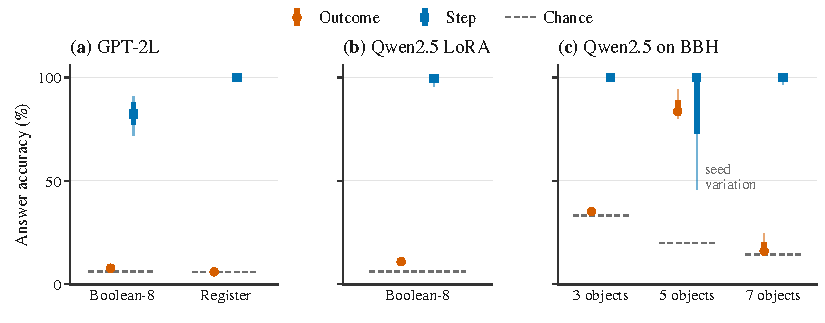
\includegraphics[width=\linewidth]{figures/main_transfer.pdf}
\caption{\textbf{Step supervision also helps beyond counting.}
Held-out answer accuracy for (a)~GPT-2L, (b)~Qwen2.5-0.5B LoRA, and (c)~Qwen2.5-0.5B LoRA on the official $250$ BIG-Bench Hard items at each object count.
Points show medians, thick intervals the interquartile range, and thin intervals the full seed range; GPT-2L Boolean-8 uses five seeds, other groups three.
Dashed segments show chance; exact values and protocols are in \cref{tab:main,app:experiments}.}
\label{fig:transfer}
\end{figure}
\paragraph{Purpose.} Synthetic state-tracking tasks test how degree structure relates to the supervision gap;
pretrained models and BIG-Bench Hard test whether the qualitative pattern transfers to a different setting.

\paragraph{Synthetic state tracking.} Boolean-8 has $4$ bits ($K=16$) and NOT, CNOT, SWAP and Toffoli gates on random wires ($n=8$); the register
machine has $(x,y)\in\mathbb Z_{17}^2$, five instructions, $n=16$ and answer $x$. Their answers put $98.9\%$ and $99.9\%$ of their
variance at degrees $\ge2$, while first occurrence keeps a degree-$1$ part at every $n$ (there $\mathbf 1[y=1]=b_1$, so $\E\|(\bm y-\bm u)_{\{1\}}\|^2\ge p(1-p)$). GPT-2L uses character tokens. \paragraph{Pretrained models and BIG-Bench Hard.} The LoRA runs test transfer of the qualitative mechanism beyond the controlled model.
On Boolean-8 (mean$\pm$SD over seeds), SmolLM2-135M LoRA reaches $9.9\pm0.2$ (outcome)
and $89.7\pm4.9$ (step); eight times the outcome budget gives $11.8\pm2.2$ (SmolLM2) and $10.0\pm0.9$ (Qwen2.5); answer-first
formats give $8.0\pm0.9$, $9.3\pm0.3$ and $10.1\pm1.0$ (GPT-2L, SmolLM2, Qwen2.5), so they do not reproduce the step benefit.



\noindent\begin{minipage}{\linewidth}
\emph{Benchmark setup and results.} Training items come from the benchmark's templates with new assignments and swaps; testing uses
the official $250$ items per size, all of which parse and rebuild exactly. Traces list every holder's item with its
option letter (``Alice has Ulysses (A)''); with item names alone, answers stayed at the letter base rate. With $m$
objects a random swap gives $\mixrate=\frac{mp-1}{m-1}$ with $p=\frac{\binom{m-1}{2}}{\binom{m}{2}}$, which is $0$, $\tfrac{1}{2}$ and $\tfrac{2}{3}$ for $m=3,5,7$, and the
share of answer variance at degrees $\le1$ is $\mixrate^{2n}+n\mixrate^{2(n-1)}(1-\mixrate^2)$: $0$, $1.56\%$ and $3.34\%$. Zero-shot accuracy is
$33.6$, $16.4$ and $11.2\%$. At three objects, outcome runs select the most common option, whose base rate is $35.2\%$.
Five objects reverse the ordering that the low-degree share predicts: outcome training reaches $80$--$94\%$ there but
$15$--$24\%$ at seven objects, whose share is larger. One of three five-object step runs fails ($46\%$ on real items, $45\%$ on
generated ones). Five objects are therefore an exception: outcome training succeeds despite less low-degree variance than seven objects.
We treat the degree calculation as a mechanistic guide, not a complete predictor of pretrained-model optimization; these LoRA runs are outside the theorem assumptions.
\end{minipage}





%=============================================================================

For the BBH spectrum measurement, we split all $6^3$ swap sequences at fixed scene, assignment and query, using the three option
logits and the LoRA up-projection Jacobian. For every task in \cref{tab:main}, $\mixrate$ is the largest singular value of the averaged
move permutation on mean-zero state vectors (\cref{def:lambda} for counting).
It determines the low-degree share for counting and BBH. For Boolean-8 and the register machine, it is only the slowest of many state modes:
the single-mode estimate $\mixrate^{2n}+n\mixrate^{2(n-1)}(1-\mixrate^2)$ gives $20\%$ and $56\%$, far above the measured
$1.1\%$ and $0.08\%$ degree-$\le1$ shares.

The summary counting rows use a zero readout and ten paired seeds with $8$k updates for modulo $2$ (mean accuracy, solved seeds in parentheses),
and $32$k updates with seeds $42$--$44$ for modulo $3$. BBH rows test on the $750$ official items, $250$ per size.

\begin{table}[H]
\centering\small
\fitwidth{\begin{tabular}{@{}llccccc@{}}
\toprule
Task & Model & $n$ & $\mixrate$ & outcome & step & chance\\
\midrule
count mod $2$ & two-block & $16$ & $0.50$ & $49.8$ ($0/10$) & $93.1$ ($8/10$) & $50$\\
count mod $3$ & two-block & $16$ & $0.66$ & $30$--$50$ & $100$ & $33$\\
first occurrence (control) & two-block & $8$--$24$ & -- & $71$--$100$ & $80$--$99$ & --\\
Boolean-8 & GPT-2L & $8$ & $0.82$ & $7.7$ & $82$ & $6.25$\\
register machine & GPT-2L & $16$ & $0.95$ & $6.3$ & $99.9$ & $5.9$\\
Boolean-8 & Qwen2.5-0.5B LoRA & $8$ & $0.82$ & $11.1$ & $98.3$ & $6.25$\\
\midrule
BBH, $3$ objects & Qwen2.5-0.5B LoRA & $3$ & $0$ & $35.2$ & $98.4$--$100$ & $33$\\
BBH, $5$ objects & Qwen2.5-0.5B LoRA & $5$ & $0.50$ & $80.0$--$94.4$ & $46$--$100$ & $20$\\
BBH, $7$ objects & Qwen2.5-0.5B LoRA & $7$ & $0.67$ & $15.2$--$24.4$ & $96.4$--$100$ & $14$\\
\bottomrule
\end{tabular}}
\caption{\textbf{Step supervision usually helps when the answer has little low-degree signal.}
Held-out accuracy (\%); ranges are over seeds. Detailed protocols and per-seed values are in the accompanying code repository.}
\label{tab:main}
\end{table}

%=============================================================================
\subsection{Joint routing runs}
\label{app:reach}

\Cref{tab:reach} uses the following protocol.
\begin{center}\small
\fitwidth{\begin{tabular}{@{}ll@{}}
\toprule
Model & two-block executor architecture (\cref{app:model}) \\
Task & counting modulo $2$, four letters, $p=\tfrac{1}{4}$ \\
Initialization & fan-in-scaled Gaussian weights, embeddings of variance $\frac{1}{d_{\mathrm{res}}}$, MLP biases of magnitude $1$--$2$,\\
& all scaled by $\initscale=0.3$; relative biases and readout zero\\
Trained & query/key maps, relative biases, readout (embeddings, values, MLPs fixed)\\
Optimizer & full-batch gradient descent, step size $2$, $4{,}096$ training prompts\\
Success & every state prediction on $16{,}384$ held-out prompts has positive margin\\
\bottomrule
\end{tabular}}
\end{center}
Of $17$ runs, $16$ solve; the remaining $n=12$ run reaches $99.95\%$ by $300$k updates. The outcome baseline uses the same
initialization, trained parameter subset, step size and data, with only the final count supervised; no outcome run
solves within $300$k updates. Implementation and per-run measurements are available in the accompanying code repository.

%=============================================================================
\section{Reproducibility}
\label{app:reproducibility}

% TODO before submission: confirm the anonymous repository URL.
\paragraph{Code.} Code, configurations, seeds, reproduction commands, numerical proof checks and per-run measurements are available at
\url{https://anonymous.4open.science/r/trace}. The accompanying code repository provides an exact implementation of the executors,
a numerical check of the reduced flow of \cref{thm:joint}, and instructions for reproducing every experiment.

\paragraph{Compute and data.} Runs use one NVIDIA A100 80GB GPU: about one minute per $8$k counting updates and fifteen minutes per
$800$-update LoRA run; exploratory runs used more compute than reported. Data are synthetic; the accompanying code repository also
contains the official BIG-Bench Hard items, unchanged. Software and assets: PyTorch 2.13 (BSD-3-Clause), Transformers 5.16 and PEFT 0.20 (Apache-2.0), SmolLM2-135M
\citep{allal2025smollm2} and Qwen2.5-0.5B \citep{qwen2025qwen25} (Apache-2.0), and BIG-Bench Hard \citep{suzgun2022challenging} (MIT).
